\documentclass[12pt, twoside, openany, abstract=on]{report}

%%%%%%%%%%%%%%% moje dodanie

\usepackage[T1]{fontenc}
\usepackage[polish, english]{babel}
\usepackage[utf8]{inputenc}
\usepackage{lmodern}
\selectlanguage{polish}
\usepackage{latexsym}
\usepackage{cite}
\usepackage{verbatim}
\usepackage{listings}
\usepackage{float}
\usepackage{lipsum} % for dummy text
\usepackage{placeins}
\usepackage[xindy]{glossaries}
\usepackage{mfirstuc}
\usepackage{listings}



\lstset{
  basicstyle=\ttfamily\small,
  columns=fullflexible,
  showstringspaces=false,
  commentstyle=\color{gray}\upshape
}
\lstdefinelanguage{XML}
{
  basicstyle=\ttfamily\tiny,
  morestring=[b]",
  morecomment=[s]{<?}{?>},
  stringstyle=\color{black},
  identifierstyle=\color{black},
  keywordstyle=\bfseries,
  morekeywords={xmlns,version,type,Count,Coefficients,,PsoParameters,Particles,ParticlesCount,ParticleType,IterationsLimitCondition,Iterations,TargetValue,TargetValueCondition,double,Epsilon,SearchSpace,Min,Max,DimensionBound,FunctionParameters,Dimension,FitnessFunctionType,NodeParameters,NrOfVCpu,Ip,Ports,int,PeerAddress}% list your attributes here
  %
}
\lstdefinestyle{sharpc}
{
  language=[Sharp]C,
  basicstyle=\ttfamily\small,
  morekeywords={var},
  frame=lr,
  rulecolor=\color{blue!30!black}
}



%%%%%%%%%%%%%%%%%%%%%%%%%%%

\usepackage[dvips]{graphicx,color,rotating}
%\usepackage[cp1250]{inputenc}
\usepackage{t1enc}
\usepackage{a4wide}
\usepackage{amsfonts}
\usepackage{amsmath}
\usepackage{enumerate}
\usepackage{verbatim}
\usepackage[MeX]{polski}
\usepackage[T1]{fontenc}
\usepackage{geometry}
\geometry{left=25mm,right=25mm,%
bindingoffset=10mm, top=25mm, bottom=25mm}
%\usepackage{amssymb, latexsym}
\usepackage{amsthm}
\usepackage{palatino}
\usepackage{array}
\usepackage{pstricks}
\usepackage{textcomp}
\theoremstyle{definition}
\newtheorem{theorem}{Twierdzenie}[section]
\newtheorem{remark}{Uwaga}[section]
\newtheorem{definition}{Definicja}[section]
\newtheorem{alg}{Algorytm}[chapter]
\newtheorem{prz}{Przypadek}[section]
\newtheorem{np}{Przykład}[section]
\newtheorem{lemma}[theorem]{Lemat}
\linespread{1.5}
\newcommand*{\norm}[1]{\left\Vert{#1}\right\Vert}
\newcommand*{\abs}[1]{\left\vert{#1}\right\vert}
\newcommand*{\om}{\omega}

\author{Paweł Kupidura, Hubert Rosiak, Kacper Trojanowski}
\title{Efektywna implementacja wybranego algorytmu optymalizacji globalnej}

\makeglossaries

\begin{document}
\begin{titlepage}
\pagestyle{empty}

\noindent
\begin{Large}
\begin{table}[t]
\centering
\begin{tabular}[t]{lcr}
 
\includegraphics[width=70pt,height=70pt]{PW} & POLITECHNIKA WARSZAWSKA & 
\includegraphics[width=70pt,height=70pt]{MiNI}\\
& WYDZIAŁ MATEMATYKI & \\
& I NAUK INFORMACYJNYCH &
\end{tabular}
\end{table}

% \vfill
\begin{center}PRACA DYPLOMOWA INŻYNIERSKA\end{center}
\begin{center}INFORMATYKA\end{center}\end{Large}
% \vfill
\begin{center}
\Huge
\textbf{Efektywna implementacja wybranego algorytmu optymalizacji globalnej}\\
\end{center}

\large Efficient implementation of a chosen global optimization algorithm

% \vfill\vfill
\vfill
\begin{center}
\Large
Autorzy:\\
\LARGE
Paweł Kupidura\\
Hubert Rosiak\\
Kacper Trojanowski
\end{center}
\vfill
\begin{center}
\Large
Promotor: mgr inż. Michał Okulewicz\\
Opiekun naukowy: prof. dr hab. inż. Jacek Mańdziuk
\end{center}
\vfill
\begin{center}
\large
Warszawa, grudzień 2016
\end{center}
\newpage
\hfill
\begin{table}[b]
\centering
\begin{tabular}[t]{ccc}
............................................. & \hspace*{100pt} & .............................................\\
podpis promotora & \hspace*{100pt} & podpis autora
\end{tabular}
\end{table}


% \maketitle
\end{titlepage}

\thispagestyle{empty}
\newpage
\pagestyle{headings}
\setcounter{page}{1}
\hyphenation{Syl-ves-tra}
\hyphenation{Syl-ves-ter-a}

\selectlanguage{polish}

\begin{abstract}
W niniejszej pracy inżynierskiej prezentujemy rozproszony system do optymalizacji funkcji umożliwiający uruchomienie obliczeń na klastrze złożonym z kilku węzłów obliczeniowych, którego bazowym silnikiem optymalizacyjnym jest algorytm Particle Swarm Optimization. Program napisany został ze szczególnym uwzględnieniem optymalizacji funkcji ciągłych z benchmarku BBOB, jednak umożliwia programiście rozszerzenie funkcjonalności do dowolnego rodzaju funkcji. System zaimplementowany został w postaci biblioteki w technologii .NET umożliwiającej dopasowanie się do sprzętu, na którym jest uruchamiana i wykorzystanie wieloprocesorowości lokalnej maszyny, a także uruchomienie obliczeń rozproszonych na wielu komputerach jednocześnie wykorzystując usługi WCF. Biblioteka pozwala też na wykorzystanie do obliczeń równoległych procesorów graficznych obsługujących technologię CUDA. Udostępnia również interfejs programistyczny, dający możliwość zaimplementowania własnej wersji algorytmu PSO, co obrazujemy przygotowując przykładową implementację dwóch wersji algorytmu. Działanie aplikacji prezentujemy poprzez wyniki testów naszej biblioteki przeprowadzonych przy użyciu platformy COCO. Wyniki wskazują na wyraźny zysk przy uruchomieniu obliczeń rozproszonych na wielu węzłach klastra, przy jednocześnie niewielkim zysku, jaki udało nam się uzyskać przy wykorzystaniu obliczeń równoległych na karcie graficznej.\\

%W niniejszej pracy inżynierskiej prezentujemy implementację wybranego przez nas algorytmu optymalizacji globalnej - Particle Swarm Optimization. Zaimplementowana przez nas biblioteka dostosowuje się do dostępnego sprzętu i pozwala na uruchomienie obliczeń na wielu procesorach, wielu maszynach i z wykorzystaniem kart graficznych. \\
%Biblioteka została stworzona w technologii .NET, wykorzystuje framework WCF do obliczeń rozproszonych oraz technologię CUDA do zlecania obliczeń na procesor graficzny wspierający tę architekturę. \\
%Do oceny naszej biblioteki wykorzystany został benchmark BBOB 2015.\\

\noindent \textbf{Słowa kluczowe.} Algorytm optymalizacyjny, PSO, CUDA

%W niniejszej pracy inżynierskiej prezentujemy stworzoną przez nas implementację algorytmu Particle Swarm Optimization. Algorytm zaimplementowany został w postaci biblioteki w technologii .NET umożliwiającej dopasowanie się do sprzętu, na którym jest uruchamiana wykorzystując wieloprocesorowość lokalnej maszyny oraz umożliwiającej uruchomienie obliczeń rozproszonych na wielu komputerach jednocześnie wykorzystując usługi WCF. Biblioteka pozwala też na wykorzystanie do obliczeń równoległych procesorów graficznych obsługujących technologię CUDA. Prezentujemy również wyniki testów naszej biblioteki m.in. na benchmarku optymalizacyjnym BBOB.
\end{abstract}


\newpage
\selectlanguage{english}
\begin{abstract}
In this paper, we present a distributed system for optimizing functions that allows user to run calculations on a cluster of several computing nodes. The base optimization algorithm used in our system is Particle Swarm Optimization algorithm. The program was written with particular emphasis on the optimization of continuous functions of Black-Box Optimization Benchmarking workshops, but allows the programmer to extend the functionality to any type of function. The system was implemented in the form of .NET library that allows adjustment to the hardware on which it runs, and the use of multiprocessing, as well as launching distributed computing on multiple computers simultaneously using a WCF service. The library allows to utilize parallel computing using GPUs that support CUDA technology. It also provides a programming interface that gives the ability to implement other versions of the PSO algorithm, which we present with a sample implementation of the two versions of the algorithm. Application performance is assesed by the results of tests conducted using the COmparing Continuous Optimisers platform. Distributed computing on multiple cluster nodes resulted with noticeable profit however we only managed to achieve small gains using parallel computing on the graphics card. \\

\noindent \textbf{Keywords.} Optimization algorithm, PSO, CUDA
\end{abstract}


\selectlanguage{polish}

\tableofcontents

%-----------Początek części zasadniczej-----------

%%%%%%%%%%%%%%%%%%%%%%%%%%%%%%%%%%%%%%%%%%%%%%%%%%%%%%%%%%%%%%%%%%%%%

\chapter{Wstęp}

Algorytmy optymalizacyjne stanowią bardzo szeroką i bogatą klasę algorytmów komputerowych, służących do znajdowania optymalnych wartości funkcji. Wśród algorytmów optymalizacyjnych znajdują się takie, które zostały opracowane z myślą o jak najszerszym zastosowaniu i dają dobre rezultaty dla wielu rodzajów problemów, jak i takie, które opracowano dla bardzo wąskiej gamy zastosowań i dzięki specjalizacji osiągają często w swojej dziedzinie najlepsze wyniki.

Jednym z algorytmów optymalizacyjnych jest algorytm Particle Swarm Optimization (PSO), należący do klasy algorytmów populacyjnych - jego populację tworzą niezależne cząsteczki poruszające się w przestrzeni rozwiązań, które komunikując się między sobą i wymieniając informacje o znalezionych rozwiązaniach, mają w zamierzeniu odkryć rozwiązanie optymalne lub jak najbardziej zbliżone do optymalnego.

W naszej pracy prezentujemy system optymalizacyjny korzystający z obliczeń rozproszonych i równoległych. Cechy algorytmu PSO takie, jak prosta koncepcja i implementacja, powodują, że wybraliśmy go jako algorytm bazowy dla naszego systemu. Co więcej, jest on algorytmem populacyjnym z dużą niezależnością cząstek i nie wymagającym sztywnej synchronizacji między nimi, co powoduje, że w klarowny sposób nadaje się do zrównoleglenia i rozproszenia obliczeń. Te cechy algorytmu wykorzystujemy w naszym systemie, tworząc klaster umożliwiający prowadzenie równoczesnych obliczeń na wielu węzłach obliczeniowych i projektując schemat komunikacji pomiędzy rojami cząstek. 

Innym z usprawnień, które postanowiliśmy wprowadzić do naszego systemu, jest możliwość przeprowadzania obliczeń na kartach graficznych. Programowanie kart graficznych stało się w ostatnich latach znacznie łatwiejsze dzięki wprowadzeniu technologii CUDA, pozwalającej programiście na tworzenie w języku zbliżonym do C rozwiązań, mogących korzystać z obliczeń równoległych na procesorach graficznych.

Ze względu na fakt, że nie istnieje jeden najlepszy algorytm optymalizacyjny, który poradziłby sobie w każdej sytuacji, zaś liczba dostępnych algorytmów optymalizacyjnych jest bardzo duża, a badania nad nimi są wciąż rozwijane, to bardzo potrzebna jest możliwość porównywania między sobą algorytmów dla różnych rodzajów problemów optymalizacyjnych. Porównanie takie umożliwiają m.in. benchmarki oparte na platformie COCO, których używamy w celu skonfrontowania jakości otrzymanego przez nas wyniku z ogólnie dostępnymi danymi dotyczącymi innych algorytmów jak i w celu ukazania zysku z rozproszenia i zrównoleglenia obliczeń.

%%%%%%%%%%%%%%%%%%%%%%%%%%%%%%%%%%%%%%%%%%%%%%%%%%%%%%%%%%%%%%%%%%%%%

\chapter{Opis teoretyczny} %[bez wspominania naszej pracy]

\section{Czym jest PSO?} %nieformalnie

PSO jest metodą rozwiązywania problemów optymalizacyjnych należącą do klasy algorytmów metaheurystycznych (ogólnych algorytmów do rozwiązywania problemów obliczeniowych, które można dostosować do konkretnego problemu), wzorowaną na spotykanym w przyrodzie zachowaniu się rojów i stad zwierząt. Po raz pierwszy przedstawiona została w pracy Eberhardta  i Kennedy’ego w 1995 r. \cite{Pso}. W ogólności polega ona na potraktowaniu potencjalnych rozwiązań zagadnienia optymalizacyjnego jako ,,cząstek'', które poruszają się w przestrzeni możliwych rozwiązań. Ruch cząsteczek odbywa się w czasie dyskretnym - w każdej iteracji głównej pętli algorytmu każda z cząstek przemieszcza się o wektor prędkości, który zależy od prędkości w poprzedniej iteracji, najlepszego dotychczas znalezionego przez sąsiadów rozwiązania (globalnego), najlepszego rozwiązania znalezionego przez daną cząstkę (lokalnego) oraz od czynnika losowego. Na poziomie praktycznym za przestrzeń rozwiązań najczęściej wybiera się n-wymiarową przestrzeń Euklidesową, zaś zagadnieniem optymalizacyjnym jest znalezienie minimum (maksimum) pewnej funkcji rzeczywistej określonej na pewnym podzbiorze tej przestrzeni. Ze względu na fakt, iż PSO jest jedynie (meta)heurystyką, szczegóły algorytmu i jego parametry można dobierać odpowiednio do konkretnego zastosowania.


\section{Definicja algorytmu} %formalnie

%zrobić tu albo wcześniej słownik PSO – co to jest (formalnie) rój, sąsiedztwo itp.
 
Pierwotna wersja algorytmu (wg. \cite{Pso}), zakładająca pełne sąsiedztwo cząstek (wszystkie cząstki w roju wzajemnie ze sobą sąsiadują) wygląda następująco:

\begin{enumerate}
\item Inicjalizacja cząstek:

\begin{enumerate}
\item Utwórz cząstki rozmieszczone losowo (według rozkładu jednostajnego) w całej przestrzeni rozwiązań;
\item Jako najlepszą znaną pozycję ustaw dla każdej z cząstek jej pozycję startową; 
\item Zaktualizuj optimum globalne znajdując pozycję cząstki o najmniejszej wartości funkcji celu; 
\item Nadaj cząstkom losowe prędkości z pewnego zakresu (według rozkładu jednostajnego; 
\end{enumerate}

\item Główna pętla algorytmu - dopóki nie został spełniony warunek stopu (określona liczba iteracji lub znalezienie wartości odpowiednio bliskiej znanemu optimum globalnemu), wykonuj:
\begin{enumerate}

\item Dla każdej z cząstek oblicz jej nową prędkość w następujący sposób:

\begin{center}

$v_{t+1} \leftarrow \omega \cdot v_t + \phi_1 \cdot r_1 \cdot p + \phi_2 \cdot r_2 \cdot g$

\end{center}

gdzie:
$v_{t+1}$ - wektor prędkości w iteracji $t+1$,\\
$v_t$ - wektor prędkości w iteracji $t$,\\
$p$ - wektor łączący obecne położenie cząstki z jej najlepszą znaną pozycją,\\
$g$ - wektor łączący obecne położenie cząstki z najlepszą globalnie pozycją,\\
$\omega$ - współczynnik bezwładności,\\
$\phi_1, \phi_2$ - ustalone przez użytkownika parametry (wagi),\\
$r_1, r_2$ - liczby z przedziału $[0,1]$ losowane w każdej iteracji\\

\item Przesuń każdą cząstkę o jej nowy wektor prędkości;
\item Dla każdej z cząstek oblicz funkcję celu w nowym położeniu i, jeżeli to możliwe, zaktualizuj najlepszą dotychczasową pozycję cząstki; 
\item Zaktualizuj optimum globalne; 
\end{enumerate}
\end{enumerate}

\begin{figure}[H]
    \centering
 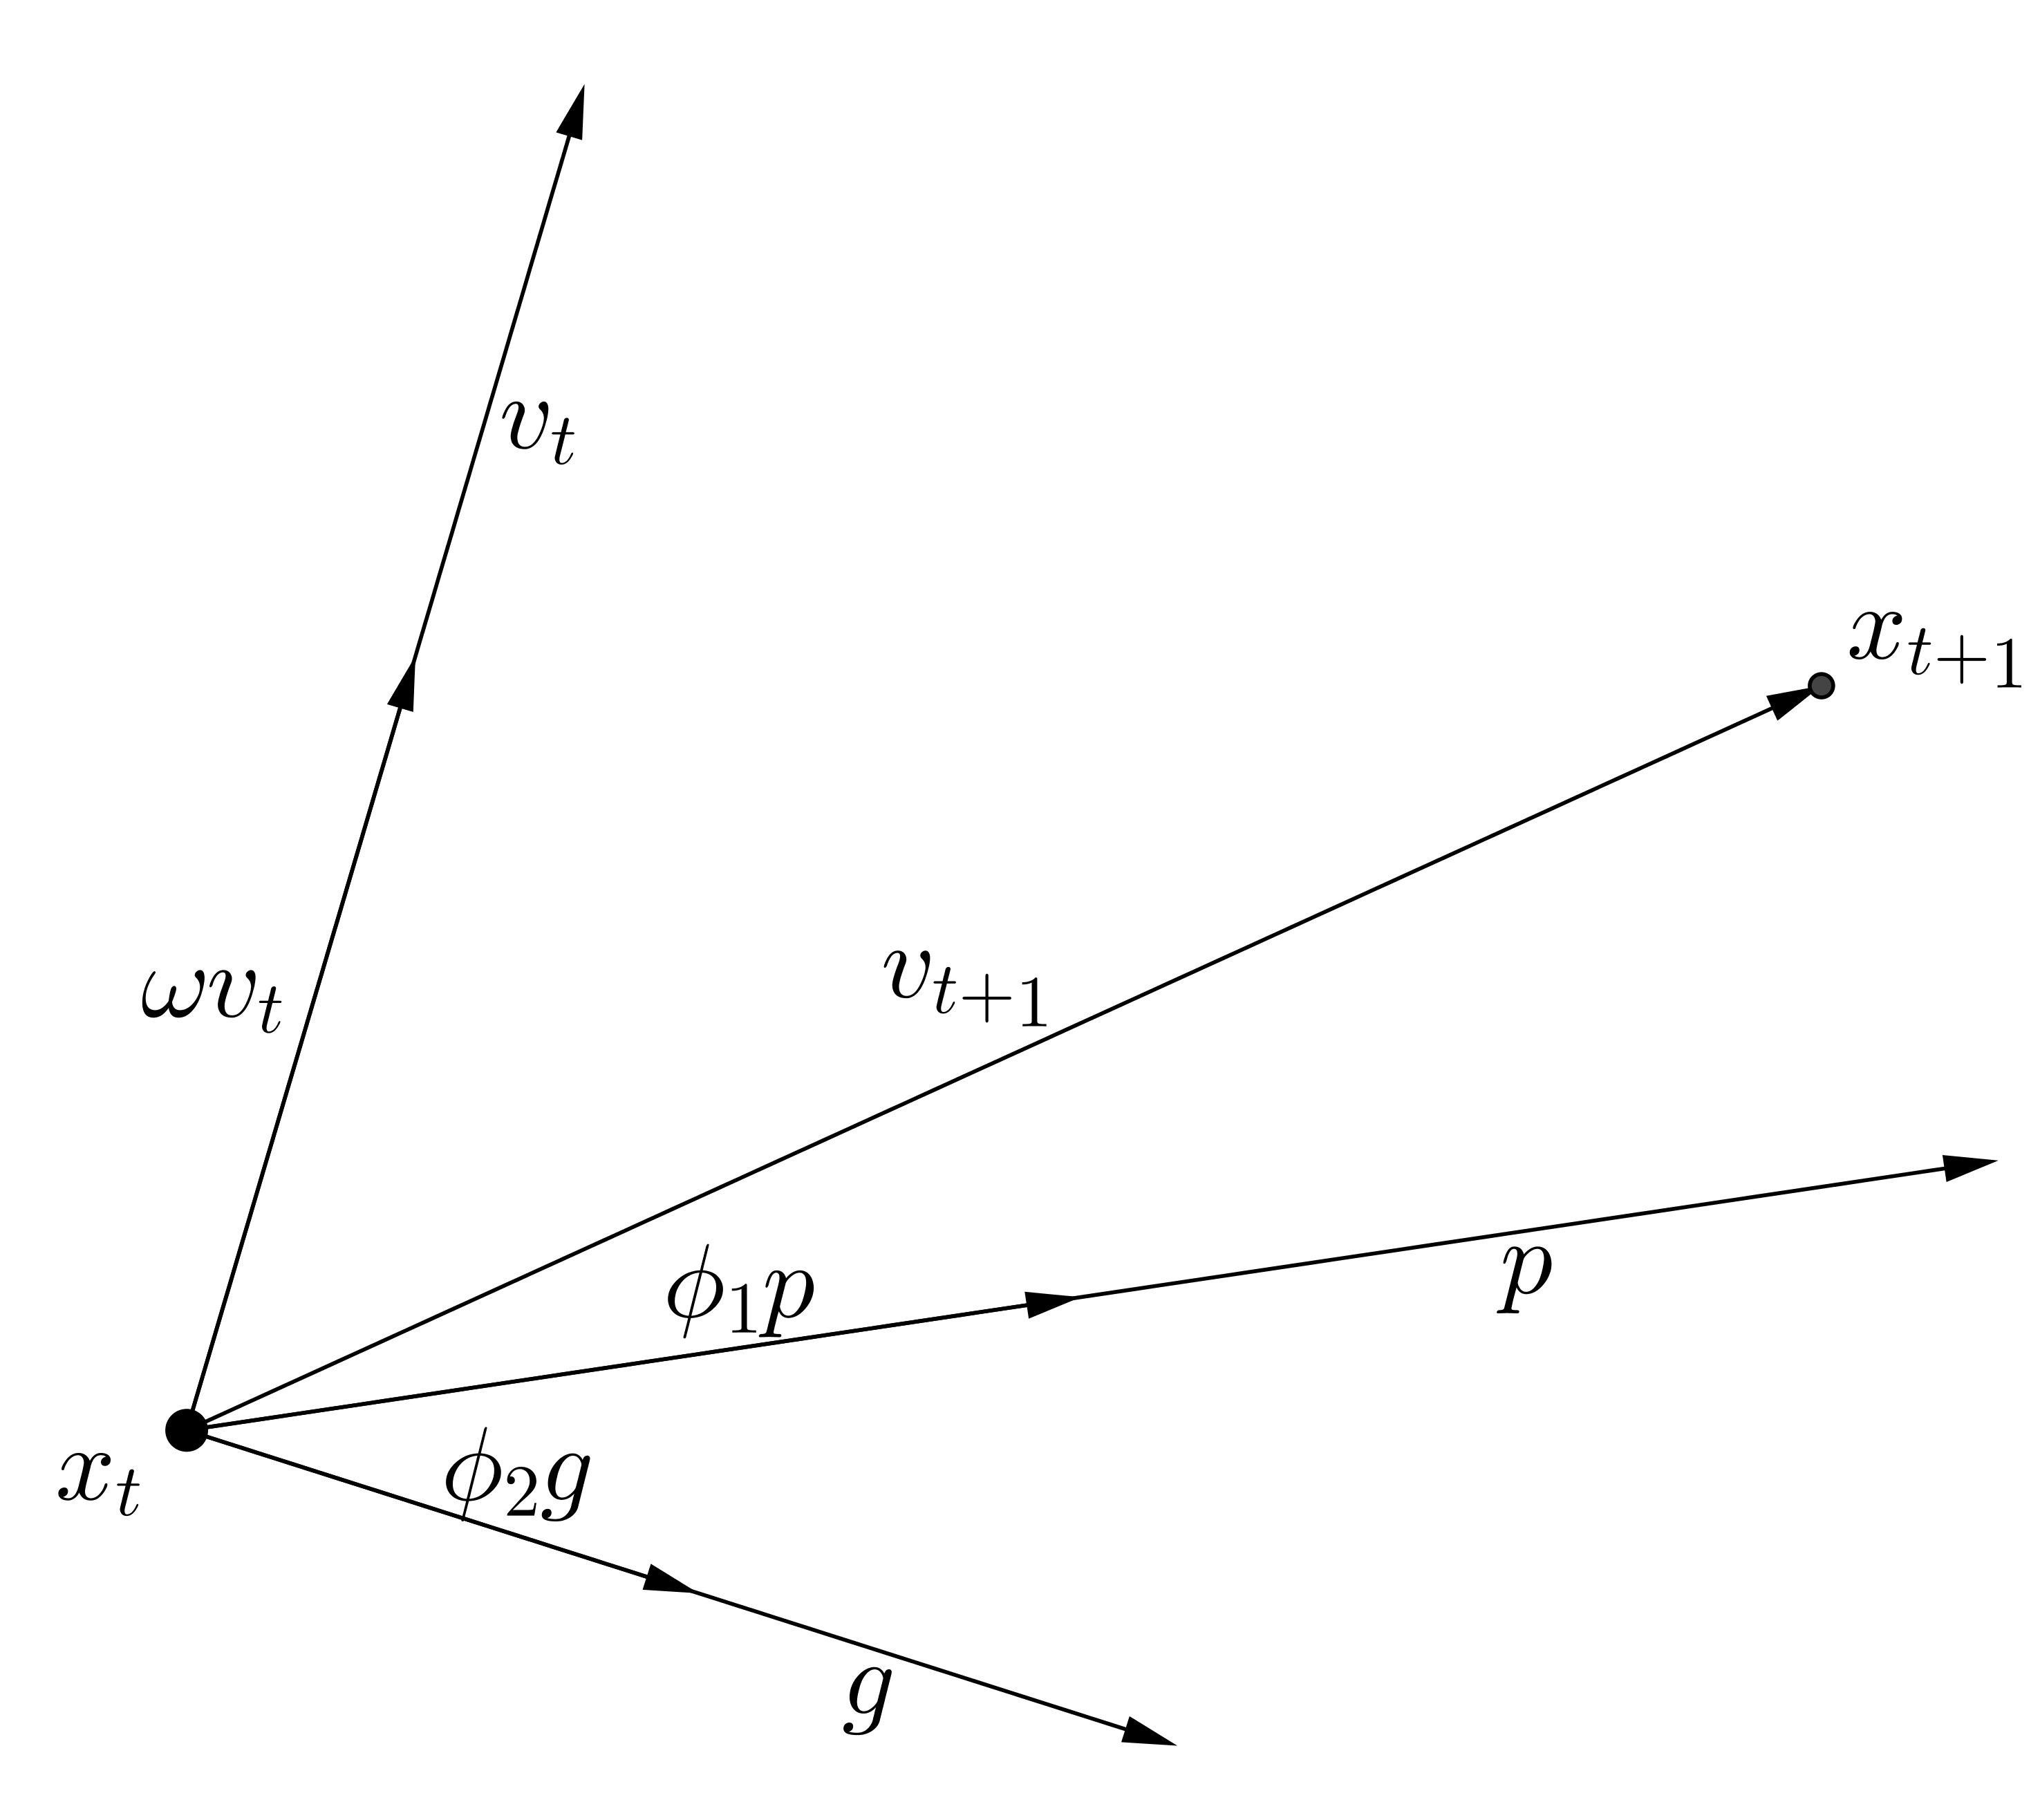
\includegraphics[scale=0.2]{PSO2D.png}
 \caption{Algorytm PSO w dwóch wymiarach}
\end{figure}

\section{Dotychczasowy stan badań nad PSO}

Od momentu powstania w 1995 r. algorytm ten zyskał popularność i szerokie zastosowanie. Był też tematem licznych prac naukowych i opracowań, mających na celu próbę jego lepszego zrozumienia i poprawy skuteczności oraz zbadanie zachowania dla wielu różnych klas problemów optymalizacyjnych.
%[do słownika problem optymalizacyjny]. 

Elastyczność definicji algorytmu sprawia, że wiele jego parametrów 
%[i procedur] 
można zmieniać i dostosowywać do aktualnych potrzeb. Skuteczność standardowej wersji PSO 
%[do słownika SPSO]
w zależności od parametrów takich, jak: wielkość roju cząstek, sposób inicjalizacji położeń i prędkości oraz ich aktualizacji w głównej pętli algorytmu czy topologia sąsiedztwa cząstek roju została zbadana w pracy \cite{SPso}. 
%[może to rozbić na parametry, a dalej o procedurach?]

%[Za \cite{ComprLearnPso}]
Dobre podsumowanie stanu badań nad PSO znajduje się w pracy \cite{ComprLearnPso}, której autorzy wspominają, iż szybko zauważono, że niektóre słabości standardowej, opisanej powyżej wersji algorytmu, można usprawnić, wprowadzając do niego pewne dodatkowe elementy, często inspirowane lub wprost pochodzące od innych algorytmów optymalizacyjnych. Powstały w ten sposób różne warianty i hybrydy algorytmu PSO.

Jedna z prostszych modyfikacji 
%[źródło?] 
wprowadza parametr ,,bezwładności $\omega$'' do wzoru wyliczającego zaktualizowaną prędkość każdej cząstki w następujący sposób:

\begin{center}

$v_{t+1} \leftarrow \omega \cdot v_t + \phi_1 \cdot r_1 \cdot p + \phi_2 \cdot r_2 \cdot g$

\end{center}

Kontrolowanie bezwładności ma umożliwiać zrównoważenie zdolności eksploatacyjnych i eksploracyjnych algorytmu 
%[do słownika]
 – duża wartości sprzyja eksplorowaniu większego obszaru, zaś mniejsza – skupienie się na bardziej lokalnym przeszukiwaniu. Bezwładność może też być dynamicznie zmieniana w trakcie wykonywania algorytmu – jej liniowe zmniejszanie się względem liczby iteracji przedyskutowano w \cite{ModPsoInertia}, zaś właściwy dobór parametrów algorytmu omówiono w \cite{ParamSelPso}. Inne, nieliniowe metody zmiany bezwładności opisano w \cite{PsoFuzzyInertia}. W pracy \cite{SelfOrgHPso} dla odmiany, parametr w ustawiany jest na 0 za wyjątkiem sytuacji reinicjalizacji.
%[co to?]
W trakcie działania algorytmu można dynamicznie modyfikować także inne jego parametry, jak np. prędkość maksymalną – wariant algorytmu implementujący jej liniowy spadek opisany został w \cite{VmaxPso}.

Duży wpływ na wydajność algorytmu ma też w oczywisty sposób topologia 
%[do słownika topologia roju] 
roju cząstek. J. Kennedy (jeden z twórców pierwotnej wersji algorytmu) stwierdził, że mniej liczne sąsiedztwo każde cząsteczki sprawdza się lepiej w przypadku bardziej złożonych problemów%[co to znaczy?]
, podczas gdy liczne sąsiedztwo działa lepiej dla prostych problemów \cite{TopologyPso}, \cite{PopStructPso}. Ciekawym rozwiązaniem jest zaproponowane w \cite{PsoNeighOp} dynamicznie dostosowywane sąsiedztwo, które stopniowo powiększa się, aż do momentu objęcia całego roju. W artykule \cite{MultiobjDynNeighPso} Hu i Eberhart zaproponowali inny sposób dynamicznego modyfikowania sąsiedztwa – w każdej iteracji algorytmu cząsteczka na nowo wybiera sobie za sąsiadów te cząstki, które są jej bliskie według pewnej metryki%jakiej?]
. Wariant UPSO (Unified Particle Swarm Optimizer) \cite{UPso} stara się połączyć globalną eksplorację z lokalną eksploatacją.
%[jak? Co to znaczy?]
Wprowadzone przez Mendesa i Kennedy’ego \cite{FullyInformedPso} Fully Informed PSO różni się od klasycznej wersji tym, że w momencie aktualizacji prędkości cząstki pod uwagę bierze się nie tylko informację pochodzącą od najlepszego sąsiada, ale, z odpowiednimi wagami, również  informacje zebrane od pozostałych sąsiadów cząstki. Wagę, jaką przypisuje się informacji od każdej z cząstek sąsiedztwa zależy m.in. od jej aktualnej wartości funkcji celu oraz rozmiaru samego sąsiedztwa. 
%[co dzięki temu zyskujemy?] [Inny wariant, „Comprehensive learning PSO.]
 Z kolei fitness-distance-ratio-based PSO (FDR-PSO) \cite{FitnessDistRatio}, wprowadza pewne dodatkowe interakcje 
%[jakie?] 
między pobliskimi cząstkami podczas aktualizacji prędkości.

Innym sposobem usprawnienia działania algorytmu, który doczekał się licznych opracowań, jest hybrydyzacji PSO, czyli próba połączenia z innymi algorytmami i technikami optymalizacji. Jednym z popularnych pomysłów jest wprowadzenie do PSO operacji znanych z algorytmów ewolucyjnych, takich jak selekcja, krzyżowanie i mutacja, w celu zachowania cech najlepszych cząstek roju, bądź też wprowadzenie większej różnorodności do populacji, mające zapobiec zbieżności do lokalnych minimów \cite{SelectionPso},\cite{HybridPsoBreedingSubpop}. Z tego samego powodu wprowadza się różne mechanizmy unikania kolizji między cząstkami \cite{CollisionAvoiding}, takie jak relokacja cząstek, które znalazły się zbyt blisko siebie \cite{PsoCriticality}. Operatory mutacji są też stosowane do mutowania 
%[?]
 parametrów algorytmu takich jak opisana wcześniej bezwładność \cite{EPso}. W pracy \cite{HybridPsoBreedingSubpop}, rój cząstek dzielony jest na mniejsze subpopulacje, zaś ,,breeding operator'' 
 %[?]
  jest stosowany w obrębie jednej z nich lub też między nimi w celu zwiększenia różnorodności roju. 
  
  Odpowiedzią na problem zbyt wczesnej zbieżności cząsteczek do minimów lokalnych, które może spowodować ominięcie minimum globalnego, jest wprowadzenie negatywnej entropii \cite{DissipativePso}. W \cite{ComputGlobOptPso} z kolei, przedstawione zostały techniki, których celem jest znalezienie jak największej liczby minimów funkcji kosztu poprzez zapobieganie poruszaniu się cząsteczek w kierunku znanych już minimów.
Jednym z innych wariantów mających poprawić wyniki otrzymywane przez PSO na funkcjach multimodalnych 
%[wielomodalnych?]
 jest tzw. cooperative PSO (CPSO-H), używające jednowymiarowych rojów do oddzielnego przeszukiwania każdego wymiaru zadanego problemu, których wyniki są następnie w odpowiedni sposób łączone.

\section{Istniejące implementacje i zastosowania PSO}

%[na podstawie \cite{EObjGeneral}]

Popularność algorytmów ewolucyjnych oraz populacyjnych, a wśród nich PSO, poskutkowała ich wykorzystaniem zarówno do badań teoretycznych jak i praktycznych zastosowań. Spowodowało to powstanie wielu implementacji tych algorytmów, z których jednak każda posiada swoje wady i ograniczenia. Jednym z podstawowych problemów wielu bibliotek jest narzucona z góry, sztywna reprezentacja osobników populacji, na których chcemy operować, czy też poddać procesowi ewolucji, jak i samych operatorów ewolucyjnych – często pozwalają one jedynie na korzystanie niewielkiego zbioru predefiniowanych reprezentacji, co zmusza do ,,spłaszczania'' bardziej skomplikowanych struktur danych do typowych postaci, na których operują istniejące biblioteki, takich jak ciągi bitów, czy tablice liczb – podejście takie może znacząco utrudnić zarówno zrozumienie, jak i rozwiązanie problemu.

Jedną z odpowiedzi na opisane wyżej problemy jest napisana w języku C++ open source’owa biblioteka EOlib (Evolving objects library), zawdzięczająca swoją elastyczność podejściu obiektowemu – każda struktura danych jak i każdy operator jest obiektem. Biblioteka zawiera kilka predefiniowanych reprezentacji, ale każdy użytkownik może stworzyć swoje własne ,,ewoluujące obiekty'', o ile tylko implementują one wymagany interfejs, tzn. zapewniają możliwość inicjalizacji, selekcji osobników oraz ich reprodukcji i mutacji (lub krzyżowania) 
%[do słownika genetycznego]
. 

Kolejną zaletą EOlib jest odejście od często stosowanego, ale ograniczającego założenia, iż funkcja celu musi być funkcją skalarną – w bibliotece tej może ona być dowolnego typu.
%[jest obiektem?]

Biblioteka Eolib jest podstawową popularnego frameworka Paradiseo (typu white-box, czyli dającego programiście wgląd w szczegóły implementacji), służącego do tworzenia metaheurystyk.
%[co to znaczy? słownik?]
Składa się on z modułów: Paradiseo-EO -  obsługującego algorytmy populacyjne, Paradiseo-MOEO – służącego do optymalizacji [wielokryteriowej], Paradiseo-MO – dla problemów z jednym rozwiązaniem, Paradiseo-PEO – narzędzia do tworzenia rozwiązań równoległych i rozproszonych.

%[może jakieś inne zastosowania lub implementacje?]

\section{Równoległe i rozproszone PSO}
%[tak ogólnie o zrównoleglaniu/rozpraszaniu obliczeń [ewolucyjnych?] - może „Obliczenia równoległe i rozproszone”]

Obliczenia rozproszone polegają na uruchomieniu jednoczesnych obliczeń na więcej niż jednym komputerze. W przypadku algorytmu PSO rozproszenie obliczeń można wykonać na wiele sposobów - na przykład za pomocą jednego wielkiego roju cząstek działającego równolegle na wszystkich maszynach lub też za pomocą większej liczby mniejszych rojów.  

%[jakie zalety mają obliczenia równoległe/rozproszone]
%...
%[jakie są trudności]
%...

%[resztę rozdziału można usunąć – wystarczy pierwszy akapit z kolejnego %działu, aby opisać równoległą naturę PSO]

Standardowa wersja algorytmu PSO wprost ze swojej natury nadaje się do zrównoleglenia obliczeń - niezależnie czy mówimy o zrównolegleniu na poziomie roju, części roju, czy też pojedynczych cząstek.
Obliczanie nowej prędkości dla każdej z cząstek zależy tylko od jej własności i własności sąsiadów z poprzedniej iteracji, zatem w oczywisty sposób potrzeby synchronizacji sprowadzają się do zaktualizowania zbioru cząstek 
%[?]
 i wyboru globalnego minimum (maksimum). 

\subsection{Stan badań nad równoległym i rozproszonym PSO}

%[za \cite{AccelParallelPso} oraz \cite{ComparisonParallelGpuPso}]

W niniejszym podrozdziale przedstawiamy obecny stan badań nad zrównolegleniem i rozproszeniem algorytmu PSO na podstawie dostępnej literatury.

Algorytm PSO jest algorytmem w naturalny sposób nadającym się do zrównoleglenia obliczeń, ze względu na fakt, że poszczególne osobniki populacji
%[?]
 są od siebie w mniejszym bądź większym stopniu niezależne i przeprowadzają samodzielne obliczenia. Dodatkowo, dla trudnych problemów optymalizacyjnych o wielu wymiarach, potrzebna liczba cząstek może być bardzo znacząca, co skłania do poszukiwania poprawy wydajności i przyspieszenia obliczeń właśnie na drodze zrównoleglenia czy rozproszenia. 
Oczywiście wraz z zaletami programowania równoległego pojawiają się charakterystyczne dla niego problemy, które należy rozwiązać, takie jak: skalowalność, synchroniczna i asynchroniczna implementacja, spójność i komunikacja sieciowa. 
%[może wyjaśnić te problemy? Chyba, że będą opisane w poprzednim rozdziale]

W pracach \cite{AccelParallelPso} oraz \cite{ComparisonParallelGpuPso} przedstawiono pokrótce niektóre z zaproponowanych do tej pory rozwiązań problemu paralelizacji algorytmu PSO. Większość z nich oparta jest na klastrach komputerów wymieniających się między sobą wiadomościami.
%[?]
Niektóre z implementacji używają popularnego standardu OpenMP. Warto wspomnieć, że analiza przeprowadzona w \cite{Pso8} wskazuje, że pewien rodzaj równoległego PSO, w którym cząstki aktualizuje się grupami, nie zawsze wymagać musi większej liczby operacji niż implementacja sekwencyjna, w której cząstki aktualizowane są jedna po drugiej, zajmując przy tym mniej czasu.

PSO jest w naturalny sposób równoległe na poziomie algorytmicznym
%[co to jest równoległość na poziomie algorytmicznym?] [embarassingly parallel]
, jednakże zaimplementowanie tej równoległości nie jest już takie oczywiste – wśród głównych problemów, z którymi należy się zmierzyć, są komunikacja %[między węzłami obliczeniowymi? Cząstkami?]
 i równoważenie obciążenia, przy czym zagadnienia te są ze sobą powiązane. W algorytmie PSO największym kosztem obliczeniowym jest zazwyczaj ewaluacja funkcji celu dla każdej cząstki. Jeżeli ewaluacja ta jest relatywnie kosztowna, koszt komunikacji można zaniedbać i pierwszoplanowym problemem staje się równoważenie obciążenia między węzłami obliczeniowymi.
 %[?] 
W przeciwnym przypadku względnie niskiego kosztu ewaluacji funkcji celu, koszt komunikacji może dominować obliczenia.

Wśród stosowanych podejść do problemu zrównoleglenia algorytmu PSO można wyróżnić dwa główne: podejście synchroniczne i asynchroniczne. W pierwszym z nich wszystkie procesory czekają na zakończenie ewaluacji funkcji celu dla wszystkich cząsteczek przed przejściem do kolejnej iteracji. Przeprowadzono wiele eksperymentów, które sugerują, że efektywność zrównoleglenia (parallel efficiency%[do słownika? Do poprzedniego rozdziału?]
) spada wraz z liczbą procesorów i jest daleka od idealnej.
%[źródło]
W celu zrównoważenia nieefektywności wynikającej z nierównego rozłożenia obliczeń, zaproponowano podejście asynchroniczne - pozwala ono każdemu wątkowi przejść niezależnie do kolejnej iteracji po ukończeniu obliczania funkcji celu. Wyniki eksperymentów pokazały znaczący wzrost efektywności w porównaniu z wersją synchroniczną. 
%[źródło]

Jednym ze sposobów zrównoleglenia obliczeń jest wykorzystanie w tym celu procesorów graficznych (GPU). Skupimy się tutaj głównie na procesorach graficznych wspierających architekturę CUDA (Compute Unified Device Architecture) \cite{CudaProgGuide} stworzoną przez firmę NVIDIA. Platforma ta zyskała bardzo dużą popularność jako prostsza i bardziej intuicyjna alternatywa dla np. standardu OpenCL.

%[może tutaj opisać architekturę CUDA, albo w ogóle gdzieś wcześniej, żeby było wiadomo, o czym mówimy w kolejnym akapicie]

W artykule \cite{GpuBasedPso} opisana została paralelizacja 
%[?]
 standardowego PSO (SPSO) na GPU z 11-krotnym przyspieszeniem względem CPU. Implementacja ta wykorzystuje topologię pierścienia, a więc umożliwia każdej cząstce komunikację z jedynie dwoma sąsiadami. Dzięki temu nie ma potrzeby równoległego poszukiwania najlepszego sąsiada podczas aktualizacji prędkości, co ogranicza konieczność komunikacja między wątkami. Z kolei rozwiązanie opisane w \cite{PsoCuda} bazuje na pomyśle utworzenia wątków GPU w liczbie równej liczbie cząstek roju pomnożonej przez liczbę wymiarów (co jednak niesie ze sobą konieczność ograniczenia maksymalnej liczby wymiarów rozważanego problemu optymalizacyjnego), który to w pewnych szczególnych przypadkach daje nawet 50-krotne przyspieszenie względem implementacji sekwencyjnej. Innym ciekawym rozwiązaniem jest zaproponowana w \cite{PsoGraphHardLocPat} hybrydyzacja algorytmu PSO z algorytmem ,,pattern search'', która na GPU może osiągnąć lepsze wyniki niż każdy z tych algorytmów z osobna. 
 %[Autorzy \cite{ComparGpuPso} porównujący warianty PSO na GPU jednak zrównoleglają jedynie ewaluację funkcji kosztu – daje to nawet 27-krotne przyspieszenie, jednakże autorzy \cite{ComparisonParallelGpuPso} uważają, że rozwiązanie to nie wydaje się być skalowalne dla większych rojów, jako, że inicjalizacja, poszukiwanie najlepszej cząstki oraz aktualizacja prędkości i położenia są wykonywane sekwencyjne.]
Artykuł \cite{BlockOccupancyGpu} bada zależność między wydajnością algorytmu PSO, a wielkością bloku wątków, uzyskując przy tym 43-krotny zysk.

%%%%%%%%%%%%%%%%%%%%%%%%%%%%%%%%%%%%%%%%%%%%%%%%%%%%%%%%%%%%%%%%%%%%%

\chapter{Zaimplementowany system optymalizacyjny}

Stworzony przez nas system optymalizacyjny składa się z jednakowych węzłów obliczeniowych, które w celu rozproszenia obliczeń mogą łączyć się w klaster, a przy dostępnych zasobach, są w stanie zrównoleglić obliczenia pomiędzy wiele wątków procesora oraz uruchomić je na karcie graficznej.


\section{Architektura węzła obliczeniowego}

Poniżej przedstawiamy najważniejsze klasy składające się na pojedynczy węzeł obliczeniowy. 

\begin{figure}[H]
    \centering
    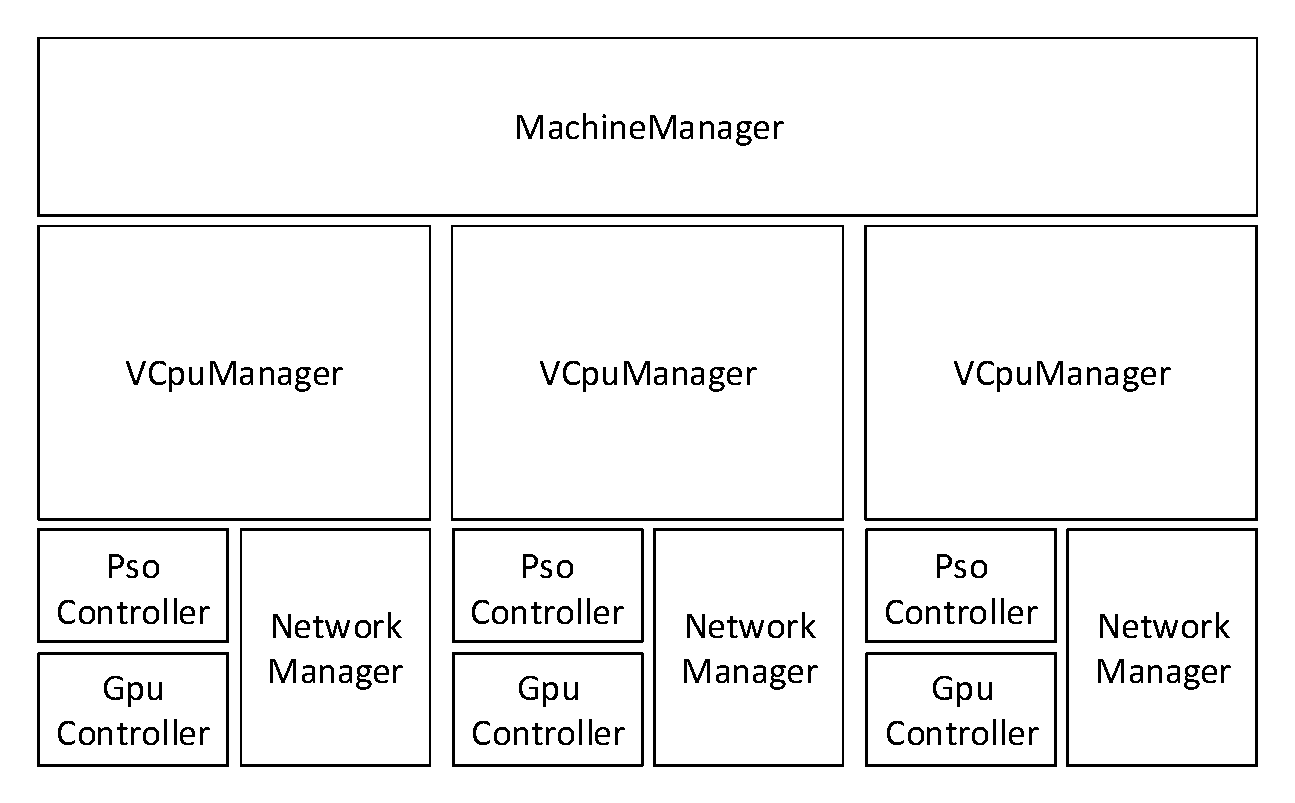
\includegraphics[scale=0.7]{WezlaArch.pdf} 
 \caption{Ogólna architektura węzła obliczeniowego}
\end{figure}

\subsection{MachineManager}
Klasa zarządzająca działaniem maszyny, umożliwiająca rozpoznanie dostępnej na komputerze liczby procesorów. Jest obiektem zaimplementowanym według wzorca fasada, odpowiedzialnym za rozpoczęcie obliczeń algorytmu (metoda \texttt{StartPsoAlgorithm}) oraz pobranie wyników (metoda \texttt{GetResult} zwracająca obiekt klasy \textit{ParticleState}), zaś za pomocą metody \texttt{Register} możemy podłączyć maszynę do klastra obliczeniowego. Obiekt klasy \textit{MachineManager} posiada tablicę \textit{VCpuManager'ów}, których liczba domyślnie odpowiada liczbie wątków procesora, lecz użytkownik może ją ręcznie zmienić.

\subsection{VCpuManager}
Klasa ta ma dwa zadania: 
po pierwsze uruchamia obliczenia jednego roju cząstek PSO, po drugie, reprezentuje pojedynczy węzeł klastra obliczeniowego i odpowiada za nawiązanie połączenia z resztą klastra. W celu oddzielenia infrastruktury sieciowej od logiki dotyczącej algorytmu PSO wykorzystuje ona interfejs \textit{IPsoController}, który zarządza warstwą logiczną klastra PSO i umożliwia m.in wywołanie metody \texttt{Run}, uruchamiającej obliczenia oraz obiekt klasy \textit{NetworkNodeManager} odpowiedzialny za komunikację pomiędzy węzłami, korzystający z technologii WCF. \textit{VCpuManager} rozpoczyna oraz kończy nasłuchiwanie na portach TCP. Stosując wzorzec obserwator zaimplementowany za pomocą funkcjonalności wydarzeń języka C\# obsługuje nowe zapytania przesyłane przez pozostałe węzły zbudowanego klastra.

\subsection{IPsoController}
Jest to interfejs odpowiedzialny za uruchomienie obliczeń algorytmu PSO na podstawie podanych parametrów wykonania.

Następujące informacje konfiguracyjne, zamknięte w klasie \textit{PsoParams}, wykorzystane są do uruchomienia algorytmu:  

\begin{itemize}
	\item Epsilon - dokładność obliczeń algorytmu
	\item FunctionParams - parametry funkcji celu: 
	
	\item Iterations - maksymalna liczba iteracji do przeprowadzenia na wątku CPU
	\item IterationsLimitCondition - wartość logiczna stanowiąca o zatrzymaniu algorytm po wykonaniu danej liczby iteracji
	\item ParticleIterationsToRestart - liczba iteracji bez poprawy położenia pojedynczej cząstki, po której dana cząstka zostanie zrestartowana, czyli jej położenie zostanie wylosowane, a najlepsza znana wartość zapomniana
	\item Particles - lista typów oraz ilości cząstek do wykorzystania
	\item PsoIterationsToRestart - liczba iteracji bez poprawy najlepszego wyniku wszystkich cząstek, po której zakończone zostanie działanie algorytmu
	\item TargetValue - wartość ekstremalna funkcji celu, do której dąży wynik algorytmu
	\item TargetValueCondition - wartość logiczna stanowiąca, czy zatrzymać algorytm po zbliżeniu się na odległość \emph{Epsilon} od \emph{TargetValue}
\end{itemize}

Parametry te przekazywane są do metody \texttt{Run}.

\subsubsection{PsoController}
Klasa \textit{PsoController} implementująca \textit{IPsoController} kontroluje wykonywanie obliczeń algorytmu PSO za pomocą obiektu \_algorithm klasy \textit{PsoAlgorithm} oraz obiektu \_cudaAlgorithm klasy \textit{GenericCudaAlgorithm}. 

Na podstawie informacji zawartych w obiekcie \textit{PsoParams}, \textit{PsoController} tworzy cząstki PSO (obiekty implementujące interfejs \textit{IParticle}) oraz funkcję celu (obiekt implementujący interfejs \textit{IFitnessFunction}), które służą następnie do uruchomienia właściwych obliczeń, co następuje w funkcji \texttt{StartAlgorithm} wywoływanej z funkcji \texttt{Run}:

\lstset{style=sharpc}
\begin{lstlisting}[frame=single]
_algorithm.Run(CancellationToken token)
\end{lstlisting}

W przypadku, gdy na maszynie dostępna jest karta graficzna spełniająca wymagania, na podstawie dostarczonych parametrów, w funkcji \texttt{PrepareCudaAlgorithm} przygotowywane jest również wywołanie algorytmu na GPU, zaś samo uruchomienie następuje w funkcji Run.

Obliczenia na CPU jak i GPU wykonywane są asynchronicznie, z możliwością przerwania ich w dowolnym momencie.

% Poniżej:
% opis części odpowiadającej za komunikację na poziome algorytmu (między rojami)

\subsection{IPsoManager}

Interfejs \textit{IPsoManager} odpowiada za komunikację pomiędzy rojami cząstek PSO znajdującymi się na różnych węzłach klastra obliczeniowego. Interfejs składa się z następujących metod:

\lstset{style=sharpc}
\begin{lstlisting}[frame=single]
void UpdatePsoNeighborhood(
NetworkNodeInfo[] allNetworkNodes, 
NetworkNodeInfo currentNetworkNode);
  
Uri[] GetProxyParticlesAddresses();

ProxyParticle[] GetProxyParticles();

event CommunicationBreakdown CommunicationLost;
\end{lstlisting}

Komunikacja pomiędzy rojami cząstek zostanie opisana w dalszej części pracy.

\subsubsection{PsoRingManager}
\textit{PsoRingManager} odpowiada za logiczne połączenie rojów na różnych węzłach obliczeniowych w pierścień (każdy rój posiada dwa roje sąsiednie).

% Poniżej:
% opis części węzła odpowiedzialnej za stworzenie klastra
% i komunikację w jego obrębie

\subsection{NetworkNodeManager}
Jest to klasa odpowiadająca za infrastrukturę sieciową klastra. Najważniejszymi polami klasy są:

\lstset{style=sharpc}
\begin{lstlisting}[frame=single]
private readonly int _tcpPort;
private ServiceHost _tcpHost;
public NodeService MyNodeService { get; set; }
public List<NodeServiceClient> NodeServiceClients
\end{lstlisting}

Po otworzeniu za pomocą metody \texttt{StartTcpNodeService} serwisu \_tcpHost nasłuchującego na porcie \_tcpPort na połączenie TCP, \textit{NetworkNodeManager} gotowy jest na przyjęcie połączenia TCP od innych węzłów. 

Interfejs sieciowy udostępniany przez węzeł obliczeniowy przedstawia klasa \textit{NodeService} opisana poniżej.

Komunikacja w drugą stronę zachodzi przy użyciu obiektów klasy \textit{NodeServiceClient}, które odpowiadają obiektom \textit{NodeService} znajdującym się na zewnętrznych węzłach.

\subsection{INodeService}
Jest to interfejs sieciowy dla węzła obliczeniowego.

\lstset{style=sharpc}
\begin{lstlisting}[frame=single]
[ServiceContract]
public interface INodeService
{
    [OperationContract] 
    void UpdateNodes(NetworkNodeInfo[] nodes);

    [OperationContract]
    NetworkNodeInfo[] Register(NetworkNodeInfo source);

    [OperationContract]
    void Deregister(NetworkNodeInfo brokenNodeInfo);

    [OperationContract]
    void StartCalculation(
    PsoParameters parameters, NetworkNodeInfo mainNodeInfo);

    [OperationContract]
    ParticleState StopCalculation();

    [OperationContract]
    void CalculationsFinished(
    NetworkNodeInfo source, ParticleState result);

    [OperationContract]
    void CheckStatus();
}
\end{lstlisting}

Dokładniejszy schemat komunikacji między węzłami klastra zostanie dokładniej opisany w późniejszym rozdziale.

\subsubsection{NodeService}
Klasa ta stanowi implementację interfejsu sieciowego węzła obliczeniowego.

\subsubsection{NodeServiceClient}
Jest to klasa, za pomocą której obiekt implementujący \textit{INodeService} jednego węzła wykonuje operacje na interfejsie sieciowym innego węzła. Technologia WCF umożliwia zaimplementowanie klienta usług sieciowych w prosty sposób - wystarczy dokonać następujące inicjalizacji:


\lstset{style=sharpc}
\begin{lstlisting}[frame=single]
Address = new EndpointAddress(tcpAddress);
Binding = new NetTcpBinding(SecurityMode.None);
ChannelFactory = new ChannelFactory<INodeService>(Binding);
INodeService Proxy = ChannelFactory.CreateChannel(Address);
\end{lstlisting}             

Na obiekcie Proxy można w tej chwili wykonywać wszystkie operacje, które implementuje interfejs sieciowy węzła o adresie tcpAddress.

\section{Komunikacja w klastrze obliczeniowym}
Komunikacja między węzłami przebiega na dwóch opisanych poniżej poziomach. Sposób połączenia węzłów w klastrze jest oddzielony od logicznego powiązania rojów PSO, dzięki czemu system umożliwia zaimplementowanie różnych topologii rojów bez konieczności ingerencji w strukturę połączeń pomiędzy węzłami.

\subsection{Komunikacja pomiędzy węzłami obliczeniowymi}
Klaster obliczeniowy jest oparty na topologii pełnej siatki, w której każdy węzeł połączony jest z wszystkimi pozostałymi i dołączany jest do sieci niezależnie od pozostałych. Każdy z węzłów jest równoważny wszystkim pozostałym, to znaczy nie istnieje centralny serwer zarządzający pracą sieci, dzięki czemu obliczenia mogą być zapoczątkowane przez dowolny z nich.

Komunikacja realizowana jest za pomocą usług WCF korzystających z protokołu sieciowego TCP. Modułem odpowiadającym za komunikację na poziomie klastra jest w każdym węźle \textit{INodeService}, który, jako serwis sieciowy, opisany jest atrybutem \texttt{[ServiceContract]}. Udostępnia on następujące usługi, z których każda posiada atrybut \texttt{[OperationContract]} i można ją wywołać zdalnie używając \textit{NodeTcpClient'a}.

Następujące funkcje muszą się znaleźć w każdej implementacji interfejsu \textit{INodeService}:

\texttt{UpdateNodes} - informuje dany węzeł obliczeniowy o zarejestrowanym nowym węźle.

\texttt{Register} - dodaje węzeł wywołujący zdalnie tę usługę do listy znanych węzłów węzła, który wykonuje usługę.

\texttt{Deregister} - usuwa węzeł wywołujący zdalnie tę usługę z listy znanych węzłów węzła ją wykonującego.

\texttt{StartCalculation} - nakazuje węzłowi rozpoczęcie obliczeń na podstawie podanych parametrów algorytmu.

\texttt{StopCalculation} - nakazuje przerwanie obliczeń i zwrócenie informacji o ich dotychczasowym wyniku.

\texttt{CalculationsFinished} - informuje o zakończeniu obliczeń na węźle, przesyłając równocześnie osiągnięty wynik.

Typowy schemat komunikacji pomiędzy węzłami jest przedstawiony poniżej.

\begin{figure}[H]
    \centering
    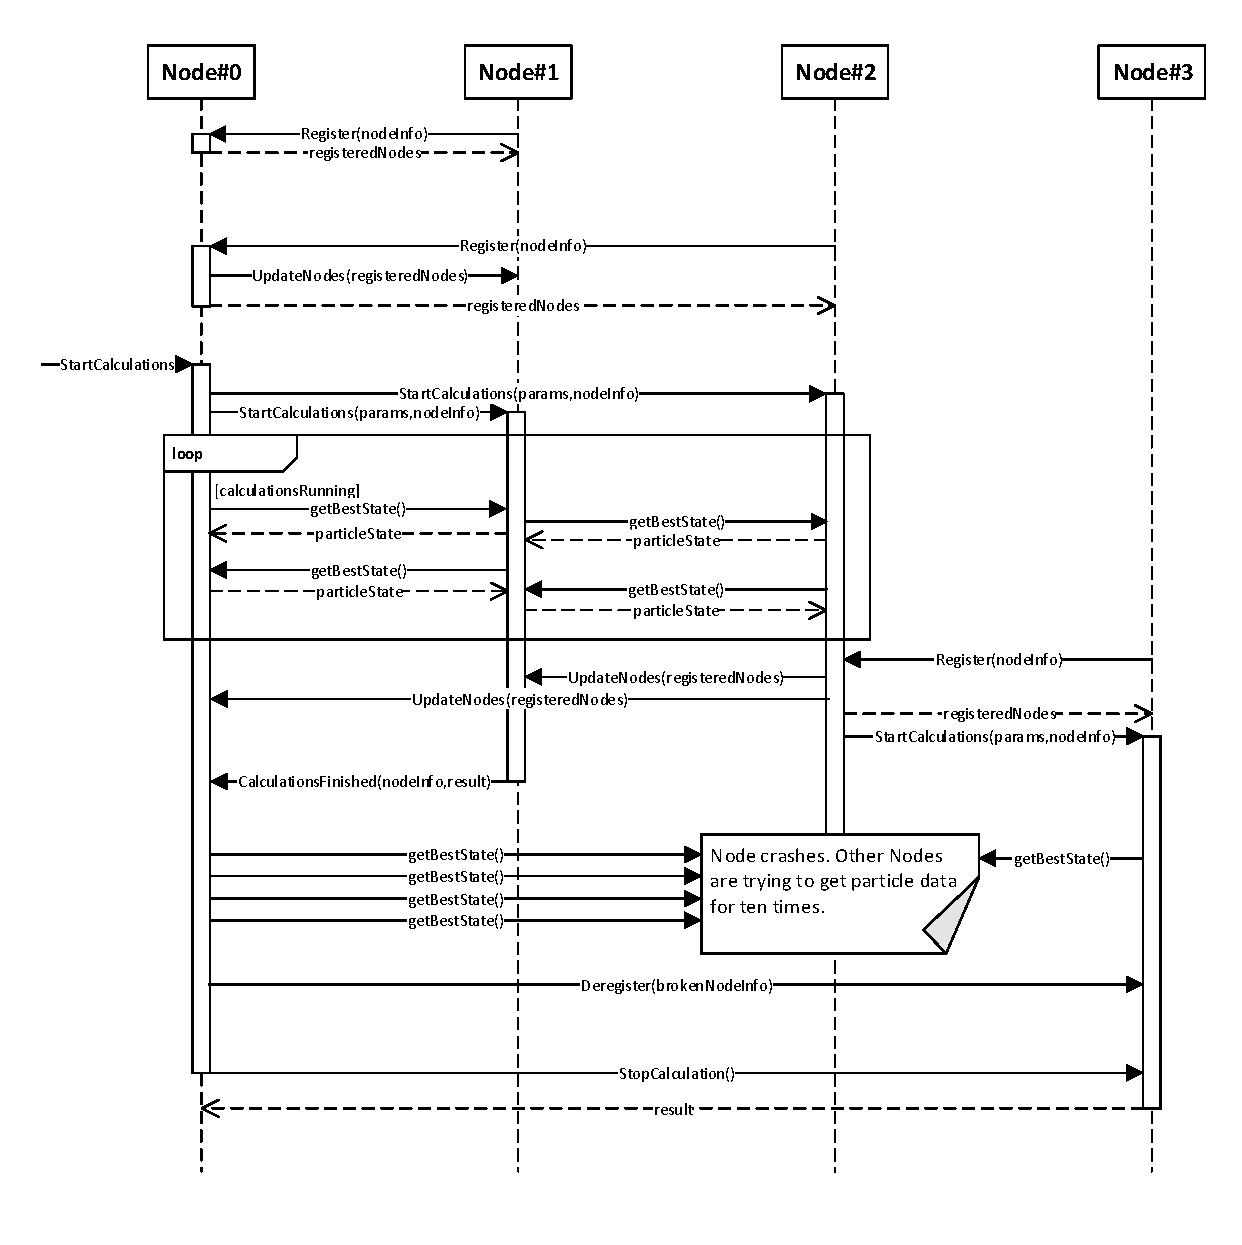
\includegraphics[scale=0.8]{communicationDiagram.pdf} 
 \caption{Diagram sekwencyjny komunikacji w klastrze obliczeniowym}
\end{figure}

%\begin{figure}[H]
%    \centering
% \includegraphics[width=1\textwidth,natwidth=610,natheight=642]%{wholeCluster.png}
% \caption{Infrastuktura klastra}
%\end{figure}

\subsubsection{Awaria}
Obliczenia są niezależne od połączeń pomiędzy węzłami klastra, dzięki czemu po awarii jednego z nich obliczenia nie są przerywane, a topologia sąsiedztwa rojów algorytmu PSO jest dostosowywana do dostępnych w danym momencie węzłów.

\subsection{Komunikacja na poziomie algorytmu PSO}
Komunikacja pomiędzy rojami PSO na różnych węzłach obliczeniwych zarządzana jest przez interfejs \texttt{IPsoManage}r, który posiadając informacje o połączonych jednostkach, definiuje sąsiedztwa pomiędzy nimi. W przypadku naszego klastra implementuje on strukturę pierścienia, w której każdy węzeł posiada dwóch sąsiadów. Połączenia pomiędzy rojami działającymi wewnątrz jednej maszyny, ale korzystające z różnych wątków procesora przebiegają w ten sam sposób co połączenia między różnymi maszynami. Wszystkie wątki, a dokładniej \texttt{VCpuManager'y} wszystkich maszyn tworzą jeden pierścień. Komunikacja pomiędzy rojami jest dwustronna. Z perspektywy cząstek wewnątrz roju, sąsiedni rój jest reprezentowany przez tzw. cząstkę proxy, która również implementuje interfejs \texttt{IParticle}, przez co nie wymaga oddzielnego traktowania - komunikacja z zewnętrznymi rojami jest przezroczysta dla innych cząstek i samego algorytmu. 

Cząstka proxy posiada odpowiadającą jej, ,,zespoloną'' z nią cząstkę proxy z innego roju.

Cząstka proxy nie wykonuje ewaluacji funkcji celu, a przekazuje jedynie najlepsze znane położenie cząstki z nią zespolonej pomiędzy rojami. Do własnego roju podaje najlepszy wynik znany cząstce proxy z roju sąsiedniego, natomiast do niej przekazuje informacje od lokalnej cząstki. Odbywa się to w momencie, gdy cząstka proxy pytana jest o najlepsze znane sobie położenie, jednakże nie za każdym razem odpytywana jest cząstka z sąsiedniego roju - dzieje się tak tylko co pewną liczbę iteracji określoną parametrem RemoteCheckInterval, który domyślnie przyjmuje wartość 200, a wprowadzony został w celu ograniczenia spadku wydajności, który zauważyliśmy, gdy komunikacja pomiędzy rojami zachodziła zbyt często.

\lstset{style=sharpc}
\begin{lstlisting}[frame=single]
public override ParticleState PersonalBest
{
	get
	{
		if (_getBestCounter == RemoteCheckInterval)
		{
			_getBestCounter = 0;
			_proxyManager.GetRemoteBestState();
		}
		_getBestCounter++;
		return _proxyManager.GetBestState();
	}
}
\end{lstlisting}


Poza informacjami przekazywanymi przez cząstki proxy, po zakończeniu obliczeń każdy z węzłów rozsyła do pozostałych informację o najlepszym znalezionym przez siebie wyniku.

Cząstka proxy komunikuje się z innymi cząstkami proxy za pomocą jeszcze jednej warstwy pośredniczącej - \textit{ProxyManagera}.

\textit{ProxyManager} jest odpowiednikiem klasy \textit{NetworkNodeManager} dla komunikacji między cząstkami - i podobnie jak \textit{NetworkNodeManager} posiadający interfejs sieciowy w postaci \textit{INodeService}, tak \textit{ProxyManager} posiada \textit{IParticleService}, który jest interfejsem sieciowej komunikacji między cząstkami i udostępnia jedną operację:

\texttt{GetBestState} - zwraca najlepszą znaną cząstce pozycję, czyli najlepszą znaną wartość wśród cząstek jej sąsiedztwa.

\begin{figure}[H]
    \centering
    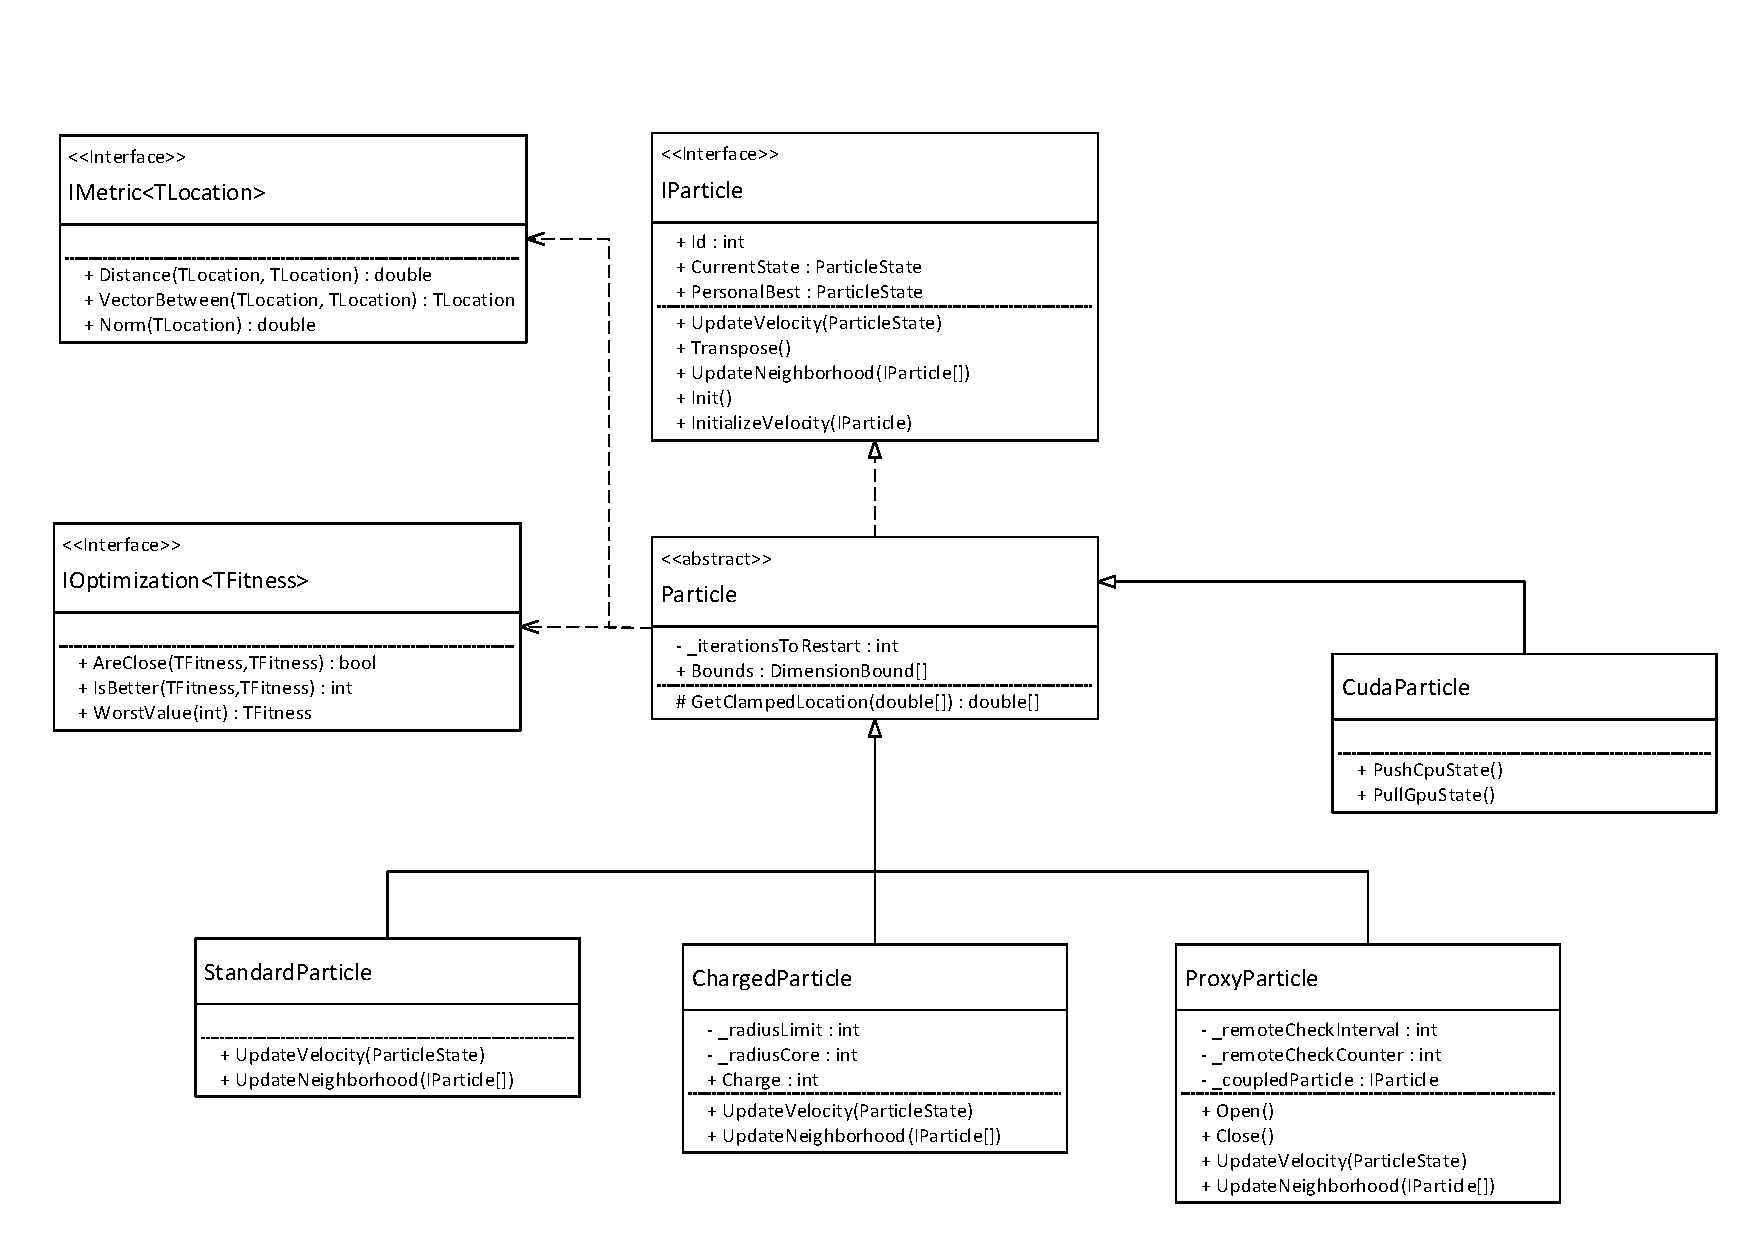
\includegraphics[scale=0.60]{particleDiagram.pdf} 
 \caption{Diagram klas związanych z cząstką PSO}
\end{figure}

\subsubsection{Wykrywanie awarii}
\textit{ProxyManager} jest jednocześnie miejscem, w którym zachodzi wykrywanie awarii. W przypadku, gdy cząstka sąsiedniego roju, z którym próbujemy się połączyć, wielokrotnie nie odpowiada na zapytanie, zgłaszane jest wydarzenie CommunicationBreakdown, a jednocześnie jako wynik zapytania zwracana jest domyślna wartość.

\lstset{style=sharpc}
\begin{lstlisting}[frame=single]
try
{
	var s = _particleClient.GetBestState();
	_particleService.UpdateBestState(s);
	_communicationErrorCount = 0;
	return s;
}
catch
{
	_communicationErrorCount++;
	if (CommunicationBreakdown != null &&
	_communicationErrorCount == communicationErrorLimit)
	{
		CommunicationBreakdown();		
	}
	return new ParticleState();
}
\end{lstlisting}

\section{Implementacja algorytmu}
Algorytm PSO w wariancie uruchamianym na CPU został przez nas zaimplementowany w jęzku C\#, co różni się od wstępnej koncepcji projektu, w której zakładaliśmy jego implementację w języku C++ oraz opakowanie go klasą w technologii .NET . Początkowo algorytm został napisany zgodnie z założeniami systemu - algorytm w języku C++ natomiast jego wrapper w języku C++/CLI. Jest to język oparty na C++ pozwalający na proste połączenie kodu natywnego C++ z kodem zarządzanym platformy .NET. Rozwiązanie takie było wystarczające dla tego modułu systemu, lecz okazało się być nadmierną komplikacją w budowie klastra oraz wykorzystaniu benchmarków BBOB.\\
W pierwszym przypadku utrudnieniem była konieczność użycia klas udostępniających usługi WCF w natywnym kodzie C++, aby  z perspektywy cząstek komunikacja między zdalnymi węzłami przebiegała w sposób jednolity do interakcji z cząstkami lokalnymi, następnie opakowanie tych cząstek w klasy języka C\# .\\
Drugi przypadek konfliktował z jednym z założeń, na podstawie którego programista mógł definiować funkcje celu w języku C\#. Spełnienie tych wymagań, osiągnęliśmy poprzez przekazywanie funkcji z maszyny wirtualnej .NET do środowiska natywnego, aby umożliwić ich wywołanie przez cząstki algorytmu. Wykorzystanie benchmarków wymagałoby dodatkowo odwrotnego opakowywania funkcji napisanych w C oraz ponadto rodziło dodatkowe komplikacje związane z odtwarzaniem funkcji dla zdalnych węzłów.

\subsection{Algorytm}
Zaimplementowanie algorytmu w języku C\# rozwiązało powyższe problemy oraz dodatkowo umożliwiło dużo przejrzystsze przekazywanie parametrów algorytmu oraz ułatwiało rozszerzanie algorytmu o nowe typy cząstek.
Sam algorytm stworzony został przez nas w taki sposób, aby był jak najbardziej generyczny ze względu na rodzaj cząstek, przez co jest odpowiedzialny jedynie za przeprowadzenie odpowiednich kroków algorytmu, których dokładna implementacja zawarta jest w cząstkach. W pętli sprawdzane są warunki stopu oraz liczone iteracje od ostatniej poprawy algorytmu, jeśli któryś z warunków zostanie spełniony, lub iteracje bez poprawy osiągną ustalony limit działanie algorytmu zostaje przerwane.

\lstset{style=sharpc}
\begin{lstlisting}[frame=single]
public IState<double[],double[]> Run(CancellationToken token)
{
	foreach(var particle in _particles)
	{
		var j = randomParticleIndex();	      
		particle.Transpose(_fitnessFunction);
	    particle.UpdateNeighborhood(_particles);
		particle.InitializeVelocity(_particles[j]);
	}
	var _currentBest = GetCurrentBest();
	_globalBest = new ParticleState(_currentBest.Location,
	_currentBest.FitnessValue);
	while (_conditionCheck())
	{
		foreach (var particle in _particles)
		{
	    	particle.Transpose(_fitnessFunction);
	    }
		foreach (var particle in _particles)
	    {
			particle.UpdateVelocity(_globalBest);
		}
	}
	return _fitnessFunction.BestEvaluation;
}
\end{lstlisting}

Możliwość przerwania obliczeń przez brak poprawy wyniku jest jednym z usprawnień względem podstawowej wersji algorytmu, które wprowadziliśmy do naszego rozwiązania, aby poprawić jego jakość. Umożliwia przeprowadzenie niezależnych restartów algorytmu po osiągnięciu wspomnianego wcześniej limitu. Analogiczne restarty pojedynczych cząstek, które w przypadku braku poprawy znalezionego osobistego optimum, rozpoczynają poszukiwania od nowa w losowym punkcie dziedziny. Wyznaczona eksperymentalnie liczba iteracji, po których następują restarty, dająca optymalne wyniki to 40 i 100 iteracji dla, odpowiednio, restartów cząstki i restartów globalnych.

\subsection{Cząstka PSO}
W naszym systemie cząstki są implementacją interfejsu \textit{IParticle}, który zawiera właściwości potrzebne do identyfikacji cząstki, określenia jej położenia obecnego i najlepszego dotychczas odwiedzonego oraz metody   aktualizujące sąsiedztwo cząstki, jej prędkość i położenie. Od implementacji cząstek zależy topologia roju oraz sposób w jaki poruszają się po przestrzeni poszukiwań. 

\subsubsection{StandardParticle}
W celu dokładniejszego opisu cząstki przestawimy przykładową cząstkę zbudowaną zgodnie z założeniami SPSO. %Czy aby na pewno
Rozszerza ona abstrakcyjną klasę \textit{Particle}, która zawiera elementy wspólne pomiędzy różnymi wersjami cząstek. Topologia jest ustalana poprzez funkcję \texttt{UpdateNeighborhood}, która wybiera sąsiadów, z którymi się komunikuje dana cząstka.
\lstset{style=sharpc}
\begin{lstlisting}[frame=single]
public override void UpdateNeighborhood(IParticle[] allParticles)
{
  Neighborhood = allParticles
   .Where(particle => particle.Id != Id)
   .ToArray();
}
\end{lstlisting}

Funkcja \texttt{UpdateVelocity} aktualizuje prędkość cząstki uwzględniając najlepsze położenia swoje oraz cząstek sąsiednich. W danym przykładzie, aby uzyskać wzrost wydajności algorytmu pojedyncza cząstka nie szuka najlepszej pozycji sąsiadów tylko otrzymuje globalną najlepszą wartość jako parametr funkcji. Jest to wartość identyczna z najlepszą wartością sąsiedztwa cząstki, gdyż w tym przypadku jest nim cały rój.

\lstset{style=sharpc}
\begin{lstlisting}[frame=single]
public override void UpdateVelocity(
IState<double[], double[]> globalBest)
{
    var toPersonalBest = Metric
      .VectorBetween(CurrentState.Location, PersonalBest.Location);
            
    var toGlobalBest = Metric
      .VectorBetween(CurrentState.Location, globalBest.Location);

    var phi1 = RandomGenerator.RandomVector(Dim, 0, Constants.PHI);
    var phi2 = RandomGenerator.RandomVector(Dim, 0, Constants.PHI);

    Velocity = Velocity.Select((v, i) => 
      v * Constants.OMEGA 
      + phi1[i] * toGlobalBest[i] 
      + phi2[i] * toPersonalBest[i]).ToArray();
}

\end{lstlisting}

Funkcja \texttt{Transpose} jest odziedziczona z klasy \textit{Particle}, ponieważ jest wspólna dla stosowanych przez nas typów cząstek. Zmienia ona obecne położenie cząstki licząc przy tym liczbę iteracji bez poprawy wartości funkcji celu. Jeśli przekroczy ona ustalony w konfiguracji algorytmu limit, cząstka jest restartowana, czyli losowane jest jej położenie początkowe oraz zapominane najlepsze dotychczas rozwiązanie.

\lstset{style=sharpc}
\begin{lstlisting}[frame=single]
public virtual void Transpose(
IFitnessFunction<double[], double[]> function)
{
  double[] newLocation;
  if (_sinceLastImprovement == _iterationsToRestart)
  {
    newLocation = randomLocation()
    _sinceLastImprovement = 0;
  }
  else
  {
    newLocation = GetClampedLocation(CurrentState.Location + Velocity);
  }
  var newVal = function.Evaluate(newLocation);
  var oldBest = PersonalBest;
  CurrentState = new ParticleState(newLocation, newVal);

  if (Optimization.IsBetter(newVal, PersonalBest.FitnessValue) < 0)
  {
    PersonalBest = CurrentState;
    _sinceLastImprovement = 0;
  }
  else
  {
    _sinceLastImprovement++;
  }
}
\end{lstlisting}

\subsection{Funkcja celu}
Funkcje celu są obiektami implementującymi interfejs \textit{IFitnessFunction}. Udostępniają one liczbę przeprowadzonych ewaluacji funkcji, najlepszą ewaluację oraz informacje o wymiarze przestrzeni poszukiwań i wartości funkcji. Funkcje są tworzone przez fabrykę funkcji \texttt{FunctionsFactory} na podstawie przekazanych do niej parametrów. W celu stworzenia odpowiedniej funkcji klient musi przekazać odpowiednią nazwę funkcji. Jest to szczególnie ważne w przypadku funkcji benchmarkowych, gdyż w nazwie zakodowany jest rodzaj funkcji oraz jej odpowiednia instancja. Dodatkowo fabryka funkcji umożliwia zapisanie danej funkcji w cache'u. Konieczność zastosowania pamięci tymczasowej była wynikiem integracji systemu z biblioteką COCO, która wymagała użycia jednej instancji funkcji celu w całym systemie.

\newpage

\section{Implementacja PSO na GPU}
\subsection{Porównanie implementacji PSO na CPU i GPU}
Implementacja na CPU, w uproszczeniu, wygląda następująco:
\begin{lstlisting}[frame=single]
while(condition) {
	foreach particle in particles:
		particle.Transpose

	foreach particle in particles:
		particle.UpdateVelocity
}
\end{lstlisting}

Zatem dopóki nie zostanie pewien warunek zakończenia, dla każdej cząstki aktualizujemy jej pozycję, a następnie dla każdej cząstki aktualizujemy jej prędkość.

Z kolei implementację algorytmu dla GPU, również w uproszczeniu, można przedstawić jako:

\begin{lstlisting}[frame=single]
while(condition) {
	RunTransposeKernel(particles)
	RunUpdateVelocityKernel(particles)
}
\end{lstlisting}

Różnica polega na tym, że aktualizacja prędkości lub pozycji odbywa się w jednym kroku dla wszystkich cząstek. Technologia CUDA umożliwia nam działanie w właśnie takim modelu - wykonanie tej samej instrukcji dla wielu danych wejściowych (SIMD - Single Instruction Multiple Data).

\subsection{Krótkie wprowadzenie do architektury CUDA}
%[Prosty opis bloków, wątków]
Opis części programu na GPU wymaga krótkiego wprowadzenia do organizacji wątków i pamięci w architekturze CUDA.

Podstawową jednostką obliczeniową 
%[to chyba niezbyt dobre określenie] 
w architekturze CUDA jest pojedynczy wątek GPU. Dzięki dostępowi do tysięcy wątków na procesorze graficznym możliwe jest stosowanie modelu SIMT (Single Instruction Multiple Threads). Każdy wątek ma dostęp do swojej lokalnej pamięci wątku. \\
Wątki zorganizowane są w wielowymiarowe bloki wątków. W zależności od wersji architektury, blok może zawierać 512 lub 1024 wątków. Poza grupowaniem wątków każdy blok wątków ma swój segment pamięci zwany pamięcią dzieloną bloku. Dostęp do tej pamięci jest dużo szybszy niż do pamięci globalnej, do której dostęp ma dowolny wątek obliczeniowy. \cite{CudaProgGuide}

\subsection{Implementacja algorytmu}
Implementacja wsparcia dla obliczeń na procesorze graficznym składa się z dwóch modułów: NativeGPU oraz ManagedGPU. Integracja między tymi modułami, napisanymi w różnych językach programowania, odbywa się poprzez bibliotekę managedCuda.

\subsubsection{managedCuda}
Biblioteka ta umożliwia na wykorzystanie potencjału kart graficznych wspierających technologię CUDA z poziomu platformy .NET. Daje ona dostęp do informacji o dostępnym sprzęcie, ułatwia zarządzanie pamięcią karty graficznej oraz umożliwia wykonywanie kerneli CUDA z poziomu kodu C\#. 

\subsubsection{NativeGPU}
Moduł zawiera implementację algorytmu PSO oraz implementacje optymalizowanych funkcji w języku CUDA. \\

Zaimplementowane funkcje nie są wykorzystywane bezpośrednio przez pozostałe moduły. Biblioteka managedCuda wykorzystuje format pośredni PTX. Pliki z kernelami kompilowane są do tego pośredniego formatu, a następnie są wczytywane do pamięci trakcie uruchomienia obliczeń z poziomu C\#. W ten sposób możemy wykorzystać te funkcje w prosty sposób z poziomu reszty systemu. \\

Kod podzielony jest na pliki zawierające kernele będące częścią algorytmu PSO, implementacje optymalizowanych funkcji oraz pomocnicze funkcje do operacji na wektorach i macierzach.

\subsubsection{update\_velocity\_kernel.cu} 
Zawiera kernel odpowiadający za wykonanie aktualizacji prędkości cząstek (pierwszy krok w głównej pętli algorytmu PSO). W przeciwieństwie do kernela, który aktualizuje lokalizacje cząstek, ten kernel jest niezależny od optymalizowanej funkcji ponieważ nie ewaluuje on optymalizowanej funkcji, przez co ma stały zestaw argumentów.

\subsubsection{Pliki dla optymalizowanych funkcji} 
Każdy z plików odpowiada różnej optymalizowanej funkcji i zawiera w sobie implementację tej funkcji w języku CUDA, kernel który inicjalizuje wartości specyficzne dla danej funkcji celu (współczynniki, macierze obrotów) oraz implementację kernela odpowiadającego za wykonanie aktualizacji lokalizacji cząstek (drugi krok w głównej pętli algorytmu PSO). Kernel aktualizujący lokalizacje różni się dla różnych optymalizowanych funkcji ze względu na różne parametry jakie te funkcje przyjmują.

\subsubsection{bbob\_generators.cuh} 
Zawiera implementacje przekształceń na wektorach i macierzach, które używane są w benchmarku BBOB, a także wiele prostych funkcji pomocniczych do działań na wektorach które były przydatne do implementacji funkcji celu lub algorytmu PSO.

\newpage

\subsubsection{ManagedGPU}
Moduł ten udostępnia API w języku C\# pozwalające na uruchomienie obliczeń na karcie graficznej oraz synchronizację obliczeń na GPU z obliczeniami na CPU. 

\subsubsection{ManagedGPU.GpuController} 
Klasa odpowiadająca za wstępną konfigurację obliczeń na GPU oraz umożliwiająca sprawdzenie możliwości maszyny obliczeniowej. Metody udostępniane przez tę klasę:
\begin{itemize}
\item \texttt{AnySupportedGpu} - sprawdza, czy na maszynie jest dostępna karta graficzna wspierająca technologię CUDA w odpowiedniej wersji. Dostęp do informacji na temat sprzętu umożliwia biblioteka managedCuda.
\item \texttt{Setup} - korzystając z otrzymanych parametrów tworzy reprezentację algorytmu (\textit{CudaAlgorithm}) oraz cząstkę proxy (\textit{CudaParticle}) która może być wykorzystana do synchronizacji obliczeń CPU i GPU. Zwrócona para obiektów jest wystarczająca do uruchomienia obliczeń na GPU samodzielnie lub w synchronizacji z CPU.
\end{itemize}

\subsubsection{ManagedGPU.CudaAlgorithm} 
Klasa która reprezentuje algorytm optymalizujący pewną funkcję. Jest to klasa abstrakcyjna - zawiera główną pętlę algorytmu i metody umożliwiające kontrolę wykonania algorytmu. Ważne metody:
\begin{itemize}
\item \texttt{Initialize} - metoda która przygotowuje zasoby do uruchomienia algorytmu na GPU. Wczytuje do pamięci odpowiedni dla optymalizowanej funkcji moduł PTX z funkcjami CUDA oraz alokuje pamięć na procesorze graficznym. Algorytm musi być zainicjalizowany przed uruchomieniem.
\item \texttt{Run} - uruchamia obliczenia na karcie graficznej. Parametrem wywołania tej metody jest token, który służy do przerwania obliczeń na GPU na żądanie. Metoda ta zawiera w sobie główną pętlę algorytmu PSO na GPU w której wywoływane są kernele CUDA 
\item \texttt{Dispose} - metoda zwalniająca zasoby zaalokowane przez instancję algorytmu. Powinna zostać wywołana po zakończeniu obliczeń.
\end{itemize}

\subsubsection{ManagedGPU.CudaParticle} 
Klasa która umożliwia synchronizację między rojem PSO na CPU i rojem na GPU. Rozszerza ona klasę \textit{Particle}, zatem może być traktowana jako zwykła cząstka z poziomu algorytmu CPU - umieszczenie takiej cząstki w roju na CPU symuluje sąsiedztwo między cząstkami na CPU i na GPU.

\newpage

\begin{figure}[H]
    \centering
 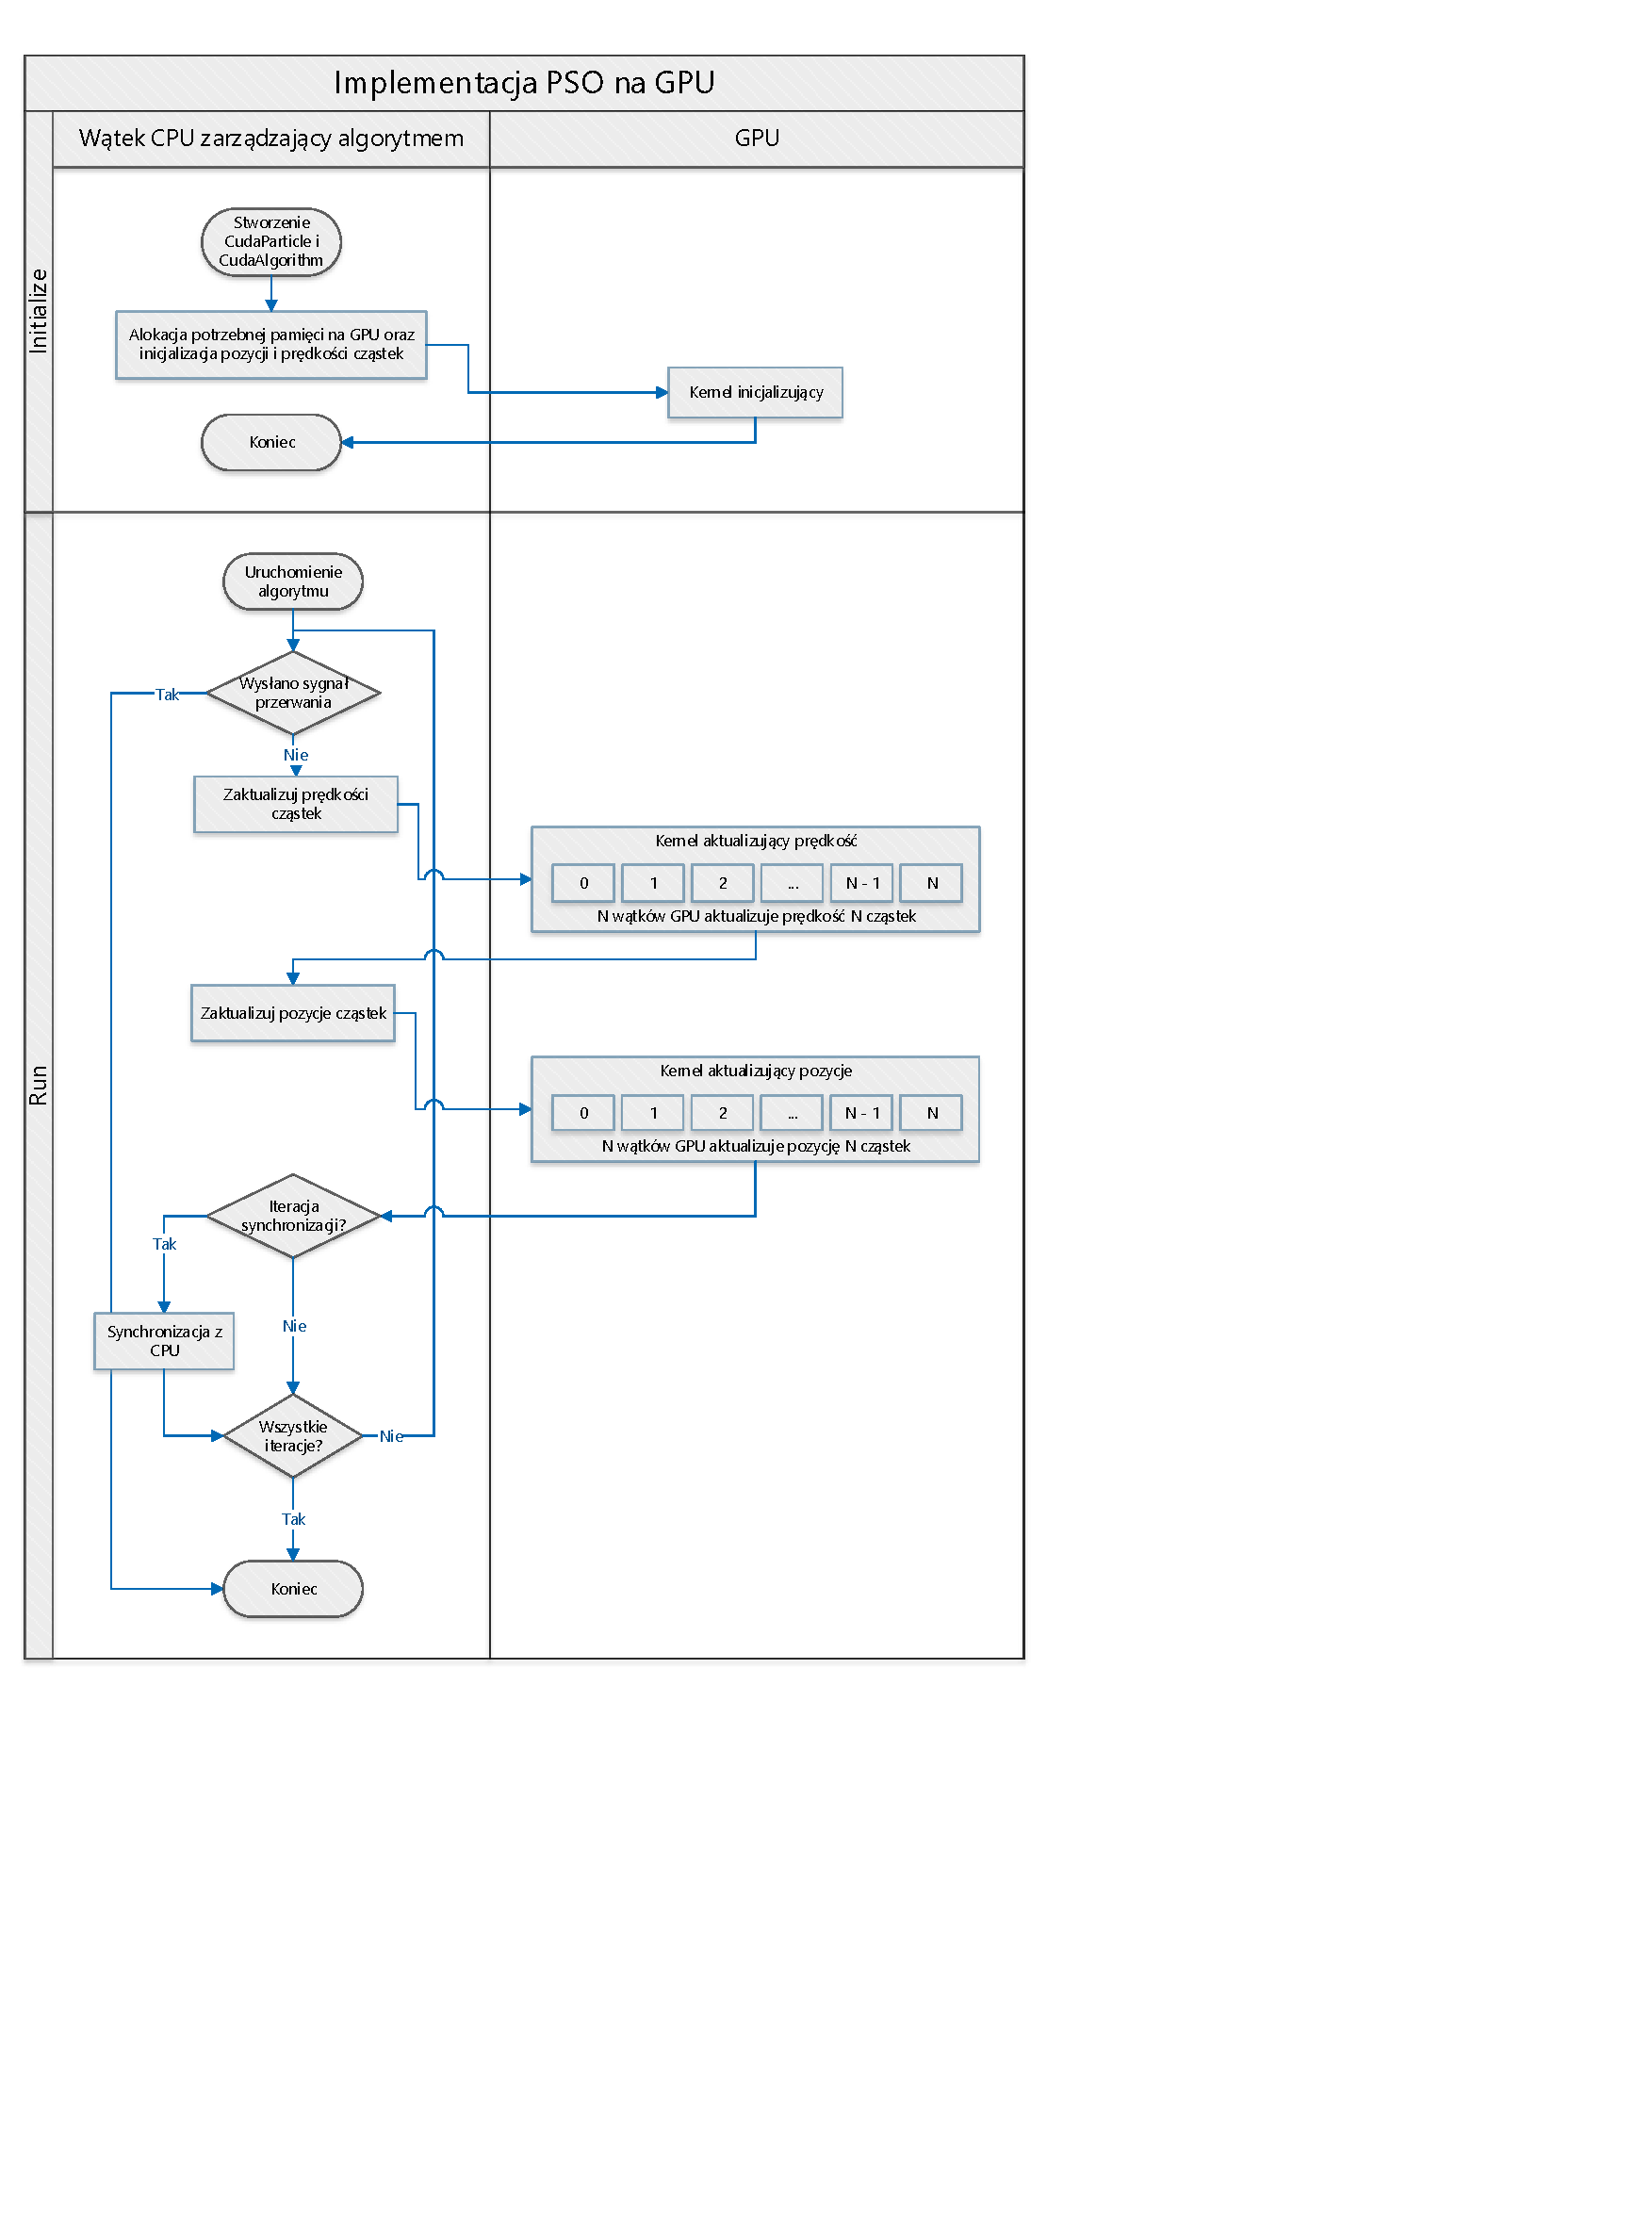
\includegraphics[width=0.9\textwidth, clip, trim=0.0cm 10cm 11cm 0cm]{gpu_diagram.pdf}
 \caption{Schemat działania algorytmu PSO na GPU}
 \label{fig:gpu}
\end{figure}

  
Jak widać na schemacie \ref{fig:gpu}, wykonywaniem obliczeń na GPU zarządza wątek CPU. \\ 
Przed uruchomieniem obliczeń obliczeń musi dojść do inicjalizacji algorytmu - kernele CUDA zostaną załadowane do pamięci oraz zostanie zaalokowana i zainicjowana pamięć na karcie graficznej. \\
Uruchomienie algorytmu powoduje wystartowanie pętli, która działa przez zadaną liczbę iteracji lub dopóki nie zostanie wysłany sygnał z zewnątrz aby przerwać obliczenia (sygnał wysyłany jest przez Token będący parametrem metody uruchamiającej algorytm). \\
W każdej iteracji tej pętli uruchamiane są dwa kernele: kernel aktualizujący prędkości cząstek oraz kernel aktualizujący pozycje cząstek. Po wykonaniu tych kroków algorytmu PSO może dojść do synchronizacji z CPU - synchronizacja zachodzi co ustaloną liczbę iteracji na GPU (w przypadku naszych testów była to empirycznie wyznaczona wartość 100 iteracji).

\subsubsection{Organizacja cząstek na GPU}
W roju cząstek na GPU stosujemy topologię pierścienia - każda z cząstek ma 2 sąsiadów, cząstkę o indeksie o jeden mniejszym i cząstkę o indeksie o jeden większym. Upraszcza to kernele po stronie CUDA i jest spójne z przyjętą topologią w pozostałej części systemu. \\
Przy wykonaniu kerneli CUDA każda cząstka obsługiwana jest przez jeden wątek. Potencjalnie jest możliwe zwiększenie stopnia zrównoleglenia poprzez delegowanie pojedynczego wątku na obsługę pojedynczego wymiaru pozycji/prędkości cząstki, ale taka organizacja wątków nie jest możliwa dla wszystkich optymalizowanych funkcji. Dlatego, dla spójności w naszej implementacji, przyjęliśmy jeden wątek GPU na jedną cząstkę PSO.

\subsubsection{Synchronizacja CPU i GPU}
Roje na GPU i CPU synchronizowane są poprzez specjalny typ cząstki \textit{CudaParticle}. Cząstka tego typu wygląda różnie w zależności od strony ją obserwującej. \\
Jeśli cząstka \textit{CudaParticle} znajdzie się w roju cząstek na CPU, zapytanie o jej cechy (np. lokalizację) zwróci cechy pewnej cząstki z roju na GPU (z czasu ostatniej synchronizacji).  \\
Od strony algorytmu na GPU cząstka ta ma cechy najlepszej cząstki z roju na CPU. Jednak wątek zarządzający algorytmem na GPU nie korzysta bezpośrednio z cząstki \textit{CudaParticle} - zamiast tego \textit{CudaParticle} i odpowiadający jej \textit{CudaAlgorithm} współdzielą obiekt \textit{CudaProxy} poprzez który udostępniają swój stan i pobierają stan z drugiej strony. \\
Synchronizacja odbywa się co ustaloną liczbę iteracji algorytmu na GPU - w iteracji synchronizacji stan pierwszej cząstki z cząstek GPU zostaje pobrany z pamięci GPU i przekazywany jest do cząstki \textit{CudaParticle}, a następnie stan najlepszej cząstki z CPU nadpisuje stan pierwszej cząstki na GPU. 
  
\subsubsection{Dodawanie własnych funkcji optymalizacyjnych}
Architektura naszego rozwiązania pozwala na dodawanie nowych funkcji do optymalizacji na GPU. \\

Aby dodać nową funkcję należy:
\begin{itemize}
\item Dodać implementację funkcji w języku CUDA wraz z odpowiednim dla niej kernelem aktualizującym pozycję cząstki.
\item Rozszerzyć klasę \textit{CudaAlgorithm} dla implementowanej funkcji rozszerzając inicjalizację pamięci o dodatkowe współczynniki dla funkcji celu (jeśli potrzebne) oraz nadpisać wywołanie kernela aktualizującego pozycję cząstki.
\item Dodać nową klasę do rejestru algorytmów ManagedCuda.CudaAlgorithmFactory z odpowiednim identyfikatorem (identyfikatory 1-24 zarezerwowane są dla funkcji z benchmarku BBOB.
\end{itemize}
 
%%%%%%%%%%%%%%%%%%%%%%%%%%%%%%%%%%%%%%%%%%%%%%%%%%%%%%%%%%%%%%%%%%%%% 
 
\chapter{Platforma COCO}

\section{Testowanie algorytmów optymalizacyjnych}
Jednym z celów naszej pracy było przetestowanie jakości implementacji algorytmu PSO na stworzonym przez nas klastrze obliczeniowym. Do tego zadania postanowiliśmy wybrać platformę COCO (COmparing Continuous Optimisers) \cite{Coco}.

Benchmarkowanie algorytmów optymalizacyjnych polega w skrócie na uruchomieniu algorytmu na przygotowanym wcześniej zbiorze problemów i zebraniu oraz przedstawieniu wyników. Nie jest to jednak tak trywialne zadanie, na jakie mogłoby wyglądać na pierwszy rzut oka m.in. ze względu na częstą trudność w dokładnej interpretacji otrzymanych wyników czy też porównaniu ich z innymi.

Odpowiedzią na te trudności jest platforma COCO umożliwiająca zautomatyzowanie procedury benchmarkowania algorytmów optymalizacyjnych. Ideą przyświecającą twórcom COCO było stworzenie środowiska zapewniającego wszystkie niezbędne do przeprowadzenie testów funkcjonalności oraz możliwość porównania danych i wyników zebranych przez różne zespoły uczonych na przestrzeni lat używających tego frameworka. 

%[why coco]

Na platformie COCO oparty jest zestaw benchmarków wykorzystany po raz pierwszy podczas warsztatów Black-Box Optimization Benchmarking (BBOB) na odbywającej się w 2009 roku konferencji GECCO.
Użyte funkcje do benchmarkowania są jawne dla użytkownika, jednakże sam algorytm, który poddajemy testom, nie ma o nich żadnej wiedzy (działają na zasadzie black-box). Lista wszystkich funkcji używanych przez BBOB dostępna jest w \cite{Coco}, jednakże my ograniczyliśmy się do pierwszych 24 funkcji (funkcje bez szumu).
Funkcje te są wybrane w ten sposób, aby dało się w jasny sposób zinterpretować na nich działanie algorytmu optymalizacyjnego. Dodatkowo nie posiadają one żadnych sztucznych regularności, które mogłyby zostać wykorzystane przez algorytm oraz są skalowalne ze względu na wymiar.

Co bardzo istotne, cały framework używa tylko jednej miary jakości algorytmu – tzw. \textit{runtime}, czyli liczby ewaluacji funkcji celu potrzebnej do osiągnięcia zadanego wyniku, czyli znalezienia wartości funkcji celu odpowiednio bliskiej wartości optymalnej. Zalety takiego podejścia są opisane w \cite{CocoPlatform}.

COCO framework składa się z biblioteki napisanej w języku C wraz z modułami odpowiedzialnymi za zbieranie i logowanie wyników, ich obróbkę (skrypty Python przygotowujące odpowiednie wykresy) oraz prezentację danych (dokumenty html oraz pliki pdf generowane na podstawie przygotowanych szablonów LaTeX) - dodatkowo dostarczone są implementacje funkcji testowych z warsztatów BBOB. Twórcy frameworka przygotowali interfejsy w językach C/C++, Java, Matlab/Octave, Python (stan w grudniu 2016) zapewniające obsługiwanie napisanych przez użytkownika algorytmów optymalizacyjnych w wymienionych językach. Niestety w chwili pisania niniejszej pracy, nie był dostępny oficjalny interfejs do języka C\#, dlatego też zmuszeni byliśmy stworzyć własny, umożliwiający komunikację z platformą COCO.

\section{Wrapper}

Stworzony przez nas wrapper ma za zadanie umożliwić wywołanie metod biblioteki COCO (CocoLibrary.c) napisanych w języku C z poziomu naszej aplikacji w języku C\#. Przy jego tworzeniu wzorowaliśmy się na dostępnym wrapperze dla języka Java wykorzystującym Java Native Interface (JNI), czyli framework umożliwiający komunikację z kodem napisanym w C/C++. 

Pierwszym zadaniem było utworzenie klas języka C\# odpowiadających klasom Javy, wykorzystywanym we wspomnianym wrapperze, a które odpowiadają pewnym strukturom języka C z biblioteki COCO. Te klasy, to:\\

\noindent \textit{Problem} - zawiera dane konkretnego problemu optymalizacyjnego.\\
\textit{Suite} - odpowiada całemu zestawowi problemów optymalizacyjnych.\\
\textit{Observer} - służy do zbierania danych w czasie wykonywania testów.\\
\textit{Benchmark} - klasa opakowująca, zawierająca w sobie obiekt klasy \textit{Suite} oraz obiekt klasy \textit{Observer}, umożliwiająca pobranie kolejnego problemu optymalizacyjnego z zestawu.\\

Klasy te stanowią interfejs benchmarku dla naszego programu - tworzone oraz inicjalizowane są w głównej pętli procedury testującej.

Między powyżej opisanymi obiektami a funkcjami z CocoLibrary.c pośredniczy jeszcze jedna warstwa, będąca prawdziwym wrapperem i zamknięta w klasie \textit{CocoLibraryWrapper}.

\subsection{Eksport / import funkcji z języka C}

Jedną z części klasy \textit{CocoLibraryWrapper} stanowią zaimportowane funkcje z CocoLibrary.c. Import funkcji jest konieczny, aby móc wywoływać je z poziomu języka C\#. Na przykładzie jednej z funkcji zaprezentujemy sposób ich importu, który wymaga następującej deklaracji:\\

\begin{lstlisting}[frame=single]
[DllImport(
"CocoLibrary.dll", 
CallingConvention = CallingConvention.Cdecl)]

unsafe static extern char* 
coco_problem_get_name(struct_pointer_t problem);
\end{lstlisting}

Umożliwia ona import funkcji o sygnaturze

\begin{lstlisting}[frame=single]
const char *coco_problem_get_name(const coco_problem_t *problem)
\end{lstlisting}

znajdującej się w pliku \textit{CocoLibrary.c}. Jak widać, aby zaimportować funkcję, należy wskazać jej źródło (w tym przypadku bibliotekę \textit{CocoLibrary.dll}) oraz sposób wywołania (w tym przypadku cdecl, czyli konwencja właściwa dla języka C). 

Dodatkowo importowana funkcja musi zostać opatrzona modyfikatorami \textit{unsafe} (umożliwiający korzystanie ze wskaźników w języku C\#) oraz \textit{extern} (wskazująca, że implementacja funkcji znajduje się w innym miejscu).

Sam import funkcji w naszej aplikacji nie wystarcza, aby uzyskać do nich dostęp. Konieczny był również ich eksport z samej biblioteki CocoLibrary.c, aby po jej skompilowaniu do CocoLibrary.dll, były one widoczne na zewnątrz. Eksport funkcji dokonuje się w następujący sposób:\\

\begin{lstlisting}[frame=single]
__declspec(dllexport) 
const char *coco_problem_get_name(const coco_problem_t *problem);
\end{lstlisting}

Zaimportowanych funkcji nie wywołujemy bezpośrednio, a za pomocą jeszcze jednej warstwy pośredniczącej, z której to korzystają już opisane wcześniej klasy \textit{Problem}, \textit{Suite}, \textit{Observer} i \textit{Benchmark}. Dodatkowa warstwa była konieczna, aby zapewnić, że funkcje eksportowane z CocoLibrary.dll wywoływane będą we właściwy sposób, jak np.:

\begin{lstlisting}[frame=single]
public static unsafe String cocoProblemGetName(long problemPointer)
        {
            char* str = coco_problem_get_name(problemPointer);
            return Marshal.PtrToStringAnsi((IntPtr)str);
        }
\end{lstlisting}

gdzie należy dokonać odpowiedniego marshallingu argumentów, czyli zmiany sposobu reprezentacji danych w pamięci na format właściwy dla transmisji do innego fragmentu programu.

\begin{figure}[H]
    \centering
    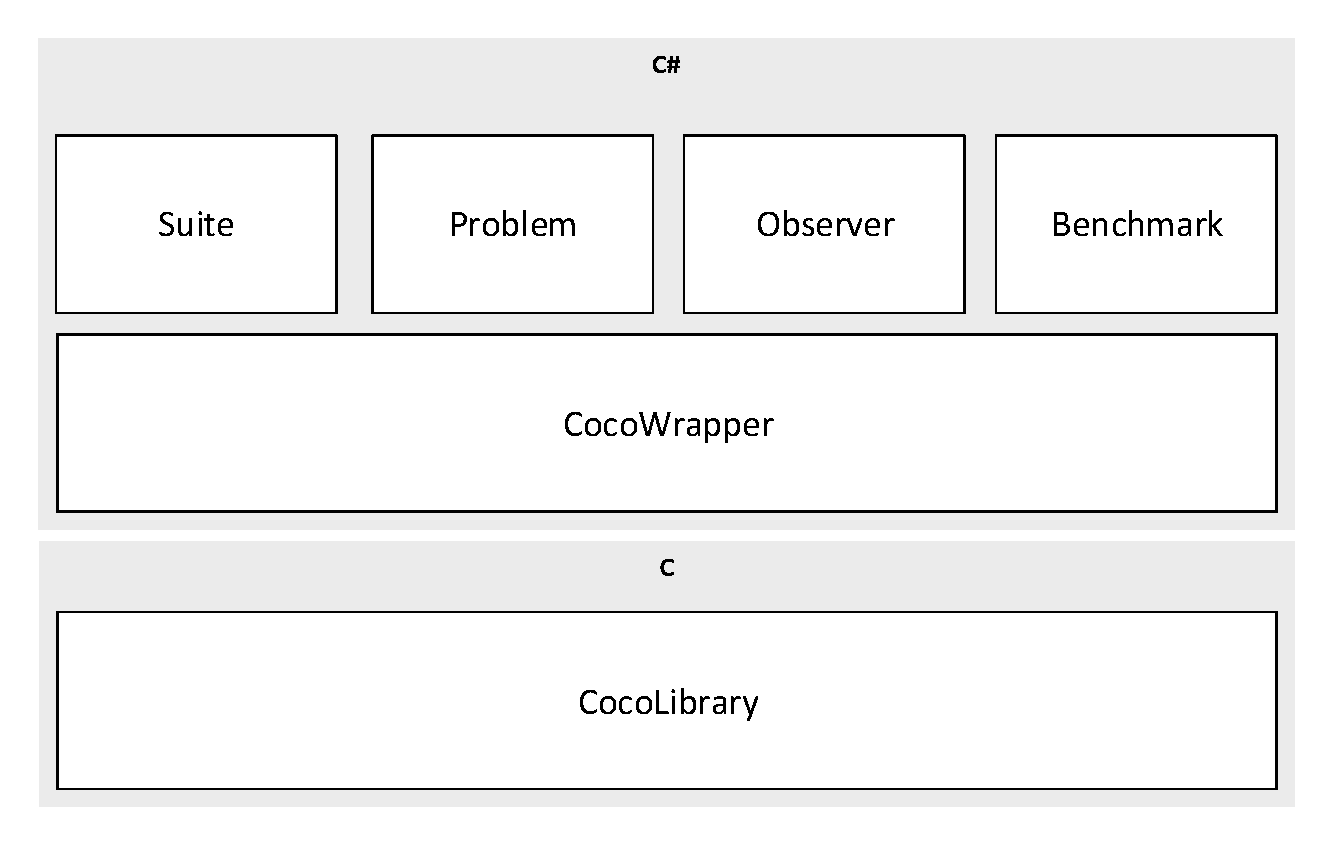
\includegraphics[scale=0.7]{wrapperDiagram.pdf} 
 \caption{Schemat wrappera}
\end{figure}

\subsection{Wykorzystanie wrappera}

Wrapper wykorzystany został w naszym programie do uruchomienia zestawu benchmarków. Inicjalizacja odpowiednich klas dokonywana jest w następujący sposób:

\begin{lstlisting}[frame=single]
var suite = new Suite("bbob", "year: 2016", "dimensions: " + dims);
var observer = new Observer("bbob", observerOptions);
var benchmark = new Benchmark(suite, observer);
\end{lstlisting}

zaś w głównej pętli programu kolejny problem do optymalizacji pobierany jest z obiektu klasy \textit{Bechmark}:

\begin{lstlisting}[frame=single]
Problem = benchmark.getNextProblem()
\end{lstlisting}

%%%%%%%%%%%%%%%%%%%%%%%%%%%%%%%%%%%%%%%%%%%%%%%%%%%%%%%%%%%%%%%%%%%%%

\chapter{Instrukcja użytkownika}

\section{Interfejs użytkownika}
Interfejs użytkownika pozwala na uruchomienie obliczeń dla jednej z zestawu predefiniowanych funkcji celu, włączając w to funkcje z benchmarku BBOB, używając zaimplementowanych typów algorytmu PSO. Umożliwia on odpowiednie dobranie parametrów funkcji celu oraz algorytmu. Za jego pomocą możliwym jest również utworzenie klastra obliczeniowego na wielu komputerach. Wybór oraz parametryzacja funkcji, algorytmu oraz konfiguracja klastra są kontrolowane przez odpowiednie pliki konfiguracyjne. 

\subsection{Klaster obliczeniowy}
Plik konfigurujący klaster obliczeniowy jest napisany w języku XML. Korzeniem dokumentu jest element o nazwie NodeParameters. 
Dziećmi elementu głównego są elementy:
\begin{enumerate}
	\item NrOfVCpu - wartość liczbowa definiująca liczbę węzłów, które zostaną utworzone przez program. Gdy przypiszemy mu wartość -1 obliczenia zostaną uruchomione na liczbie wątków dopasowanej do procesora.
	\item Ip - adres interfejsu sieciowego maszyny, z którą będą mogły połączyć się pozostałe wątki klastra
	\item Ports - tablica integerów z numerami portów, na których nasłuchiwać będą usługi WCF
	\item PeerAddress - element zawierający adres węzła, do którego aplikacja powinna się podłączyć. Powinien zostać pominięty w przypadku, gdy użytkownik nie ma zamiaru łączyć się z innymi jednostkami
\end{enumerate}
Przykładowy plik konfiguracyjny klastra:
\lstset{language=XML}
\begin{lstlisting}[frame=single]
<?xml version="1.0" encoding="utf-8"?>
<NodeParameters xmlns:xsi="http://www.w3.org/2001/XMLSchema-instance" xmlns:xsd="http://www.w3.org/2001/XMLSchema">
  <NrOfVCpu>1</NrOfVCpu>
  <Ip>25.123.241.71</Ip>
  <Ports>
    <int>8000</int>
  </Ports>
  <PeerAddress>net.tcp://25.123.244.149:8000/NodeService</PeerAddress>
</NodeParameters>
\end{lstlisting}

\subsection{Algorytm PSO}
Plik konfigurujący algorytm PSO oraz funkcję celu również napisany jest w języku XML. Korzeniem dokumentu jest element o nazwe PsoParameters. 
Dziećmi elementu głównego są elementy:
\begin{enumerate}
	\item Particles - tablica definiująca liczbę oraz rodzaj cząstek użytych do obliczeń
	\item IterationsLimitCondition, Iterations - wartość logiczna określająca czy warunek stopu ze względu na liczbę iteracji powinien być zastosowany oraz liczba iteracji do wykonania
	\item TargetValueCondition, TargetValue, Epsilon - wartość logiczna określająca czy warunek stopu ze względu na osiągnięcie optimum powinien być zastosowany, optimum funkcji celu do wykonania oraz dokładność z jaką powinno być osiągnięte
	\item FunctionParameters - definiujące parametry funkcji celu. Dziećmi tego elementu są:
	\begin{enumerate}
		\item FitnessFunctionType - typ funkcji celu. Id funkcji w przypadku funkcji z benchmarku BBOB
		\item Dimension - wymiar funkcji
		\item Coefficients - współczynniki funkcji
		\item SearchSpace - tablica zawierająca dolną i górną granicę dziedziny poszukiwań
	\end{enumerate}
	\item GpuParameters - definiujące parametry roju GPU. Dziećmi tego elementu są:
	\begin{enumerate}
		\item UseGpu - wartość logiczna decydująca o tym, czy używać GPU w obliczeniach
		\item ParticlesCount - liczba cząstek na GPU
		\item Iterations - maksymalna liczba iteracji do wykonania na GPU
	\end{enumerate}
	\item PsoIterationsToRestart - liczba iteracji algorytmu bez poprawy wyniku, która musi zostać wykonana zanim zostanie on zatrzymany
	\item ParticleIterationsToRestart - liczba iteracji algorytmu bez poprawy wyniku danej cząstki, po której cząstka zostanie zrestartowana

\end{enumerate}
\clearpage
Przykładowy plik konfiguracyjny algorytmu PSO:
\lstset{language=XML}
\begin{lstlisting}[frame=single]
<?xml version="1.0" encoding="utf-8"?>
<PsoParameters xmlns:xsi="http://www.w3.org/2001/XMLSchema-instance"
 xmlns:xsd="http://www.w3.org/2001/XMLSchema">
  <Particles>
    <ParticlesCount>
      <ParticleType>Standard</ParticleType>
      <Count>6</Count>
    </ParticlesCount>
  </Particles>
  <IterationsLimitCondition>true</IterationsLimitCondition>
  <Iterations>1000</Iterations>
  <TargetValueCondition>false</TargetValueCondition>
  <TargetValue>0</TargetValue>
  <Epsilon>1e-12</Epsilon>
      <FunctionParameters>
        <FitnessFunctionType>quadratic</FitnessFunctionType>
        <Dimension>2</Dimension>
        <Coefficients>
          <double>1.0</double>
          <double>1.0</double>
        </Coefficients>
        <SearchSpace>
          <DimensionBound>
            <Min>-5</Min>
            <Max>5</Max>
          </DimensionBound>
    	  <DimensionBound>
            <Min>-5</Min>
            <Max>5</Max>
          </DimensionBound>
        </SearchSpace>
      </FunctionParameters>
</PsoParameters>
\end{lstlisting}
\section{CocoClusterApp}
CocoClusterApp jest aplikacją kliencką naszej biblioteki umożliwiającą uruchomienie benchmarków COCO we wszystkich wspieranych przez nasz system konfiguracjach. Ustawienie programu przebiega niemal identycznie jak w przypadku opisanym powyżej, lecz aplikacja nadpisuje niektóre z ustawionych wartości. Są to:

\begin{itemize}
\item IterationsLimitCondition - zawsze ustawiany na true
\item Iterations - limit iteracji jest ustawiany na podstawie wywołania programu
\item TargetValueCondition - zawsze ustawiane na false, ponieważ benchmarki są zaimplementowane wg. doktryny black-box, czyli algorytm nie zna optimum funkcji
\item FunctionParameters - poszczególne funkcje benchmarków są wczytywane i następnie ustawiane są jej parametry
\end{itemize} 
\subsection{Wywołanie programu}
  Wywołanie programu następuje za pomocą poniższej komendy

\lstset{style=sharpc}
\begin{lstlisting}[frame=single]
.\CocoClusterApp.exe <Dim1[,Dim2,Dim3...]>\
   <FunctionsFrom> <FunctionsTo> <Budget>
\end{lstlisting}
gdzie pierwszym parametrem jest oddzielona przecinkami lista wymiarów ze zbioru \{2,3,5,10,20,40\} , drugim i trzecim są liczby definiujące przedział optymalizowanych funkcji od 1 do 24, natomiast ostatnim jest budżet algorytmu, który dla każdej optymalizowanej funkcji jest ilorazem liczby jej ewaluacji i wymiaru.

\subsection{Wyjście programu}
W trakcie działania programu na ekran konsoli wypisywana jest nazwa ostatnio zakończonej funkcji, liczba ewaluacji przeprowadzonych na danym węźle (bez GPU), liczba restartów algorytmu oraz najlepsza osiągnięta wartość.\\

Szczegółowe dane dotyczące przebiegu algorytmu zapisywane są przez bibliotekę COCO w folderze \textbf{./exdata/<ParticleIterationsToRestart>P\_<PsoIterationsToRestart>G}. W folderze tym, dla każdej funkcji znajduje się folder z danymi oraz plik o rozszerzeniu .info . Plik info zawiera dla każdego wymiaru dwie linijki. W pierwszej są to Id funkcji, wymiar, precyzja oraz nazwę algorytmu. W drugiej linii w pierwszej kolumnie zawarta jest ścieżka do pliku ze szczegółowym przebiegiem algorytmu, natomiast w kolejnych kolumnach przedstawiony jest numer instancji funkcji, numer ewaluacji w której osiągnięto dla niej najlepszy wynik oraz jego dokładność. 
Plik, do którego kieruje pierwsza kolumna, znajduje się we wspomnianym wcześniej folderze. Można z niego odczytać numery ewaluacji, dla których PSO odnalazło dotychczas najniższą wartość funkcji, dokładną wartość minimum funkcji, oraz znalezione przez algorytm punkty (współrzędne wraz z dokładnością). Struktura pliku opisana jest w jego nagłówku. 


\chapter{Wykorzystane biblioteki i technologie}
Żadna z wykorzystanych przez nas bibliotek nie nakłada ograniczeń na sposób licencjonowania projektu. \\

Wykorzystane przez nas biblioteki:

\begin{itemize}
\item managedCuda, licencja LGPL, https://github.com/kunzmi/managedCuda
\item Chronometer, licencja MIT, https://github.com/narkhedegs/Chronometer
\item CUDA Toolkit, licencja NVIDIA pozwala na wykorzystanie w naszym projekcie, https://developer.nvidia.com/cuda-toolkit
\item COCO (Comparing Continuous Optimizers), licencja BSD, \\
https://github.com/numbbo/coco/
\end{itemize}

\section{Wymagania techniczne}

Do uruchomienia aplikacji niezbędny jest komputer z systemem operacyjnym Windows z
platformą .NET 4.5. W celu uruchomienia obliczeń na procesorze graficznym wymagana jest karta graficzna wspierająca wersję (compute capability) 2.0 architektury CUDA.
Użytkownik w celu zestawienia klastra komunikującego się przez zewnętrzne interfejsy sieciowe powinien posiadać uprawnienia administratora. Należy pamiętać również, o zezwoleniu aplikacji na nawiązywanie połączeń internetowych (dodać wyjątek do firewalla).


\chapter{Testy}

Poniżej znajdują się wyniki i interpretacja testów naszej biblioteki przeprowadzonych przy użyciu platformy COCO oraz zestawu benchmarków z warsztatów BBOB.

\section{Plan testów}
Bazową konfiguracją, względem której oceniamy wyniki pozostałych testów, jest rój złożony ze standardowych cząstek uruchomiony na jednym węźle obliczeniowym bez użycia GPU.\\

Testów dokonujemy na trzech płaszczyznach:

\begin{enumerate}
\item{Dokonujemy hybrydyzacji algorytmu PSO, zamieniając połowę cząstek roju na cząstki naładowane (pochodzące z Charged PSO).}

\item{Wspomagamy algorytm obliczeniami równoległymi na karcie graficznej, na której znajduję się dużo większy rój złożony ze standardowych cząstek.}

\item{Uruchamiamy obliczenia na klastrze obliczeniowym, złożonym z różnej liczby węzłów posiadających standardowy rój cząstek.}
\end{enumerate}

\begin{table}[t]
\caption{Tabela przedstawiająca przeprowadzone przez nas eksperymenty}
\label{Zestawienie testów}
\setlength{\tabcolsep}{15pt}
\begin{tabular}{c c|c|c|c|}
  \cline{3-5}
  & & \multicolumn{3}{|c|}{Liczba cząstek}  \\
  \hline
   \multicolumn{1}{|c|}{Id.} & L. węzłów & Standard CPU & Charged CPU & Standard GPU \\ 
  \hline
  	\multicolumn{1}{|c|}{1} & 1 & 40 & 0 & 0 \\
  \hline
    \multicolumn{1}{|c|}{2} & 1 & 20 & 20 & 0 \\
  \hline
    \multicolumn{1}{|c|}{3} & 1 & 40 & 0 & 640 \\
  \hline
    \multicolumn{1}{|c|}{4} & 2 & 40 & 0 & 0 \\
  \hline
    \multicolumn{1}{|c|}{5} & 4 & 40 & 0 & 0 \\
  \hline
\end{tabular} 
\end{table}
\subsection{Konfiguracje testowe}


\subsubsection{Pojedynczy węzeł obliczeniowy}
Testów porównujących hybrydyzację algorytmu PSO ze standardowym algorytmem dokonujemy na pojedynczym węźle obliczeniowym, na którym znajduje się rój 40 cząstek, z których połowa stanowią cząstki naładowane.

\begin{figure}[H]
    \centering
    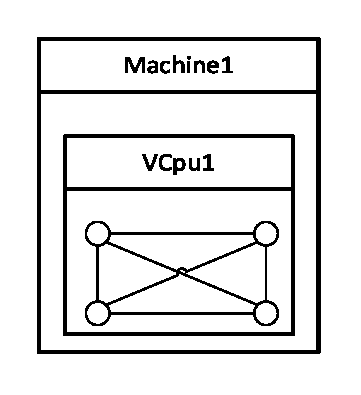
\includegraphics[scale=1]{klasterBbobNoGPU1Node.pdf} 
 \caption{Struktura pojedynczego węzła obliczeniowego z rojem złożonym z 40 cząstek}
\end{figure}

\subsubsection{Pojedynczy węzeł obliczeniowy z GPU}
Do zmierzenie zysku, jaki daje użycie obliczeń na karcie graficznej używamy standardowej wersji PSO na jednym węźle z 40 standardowymi cząstkami, którą wspomaga złożony z 640 cząstek rój na karcie graficznej.

\begin{figure}[H]
    \centering
    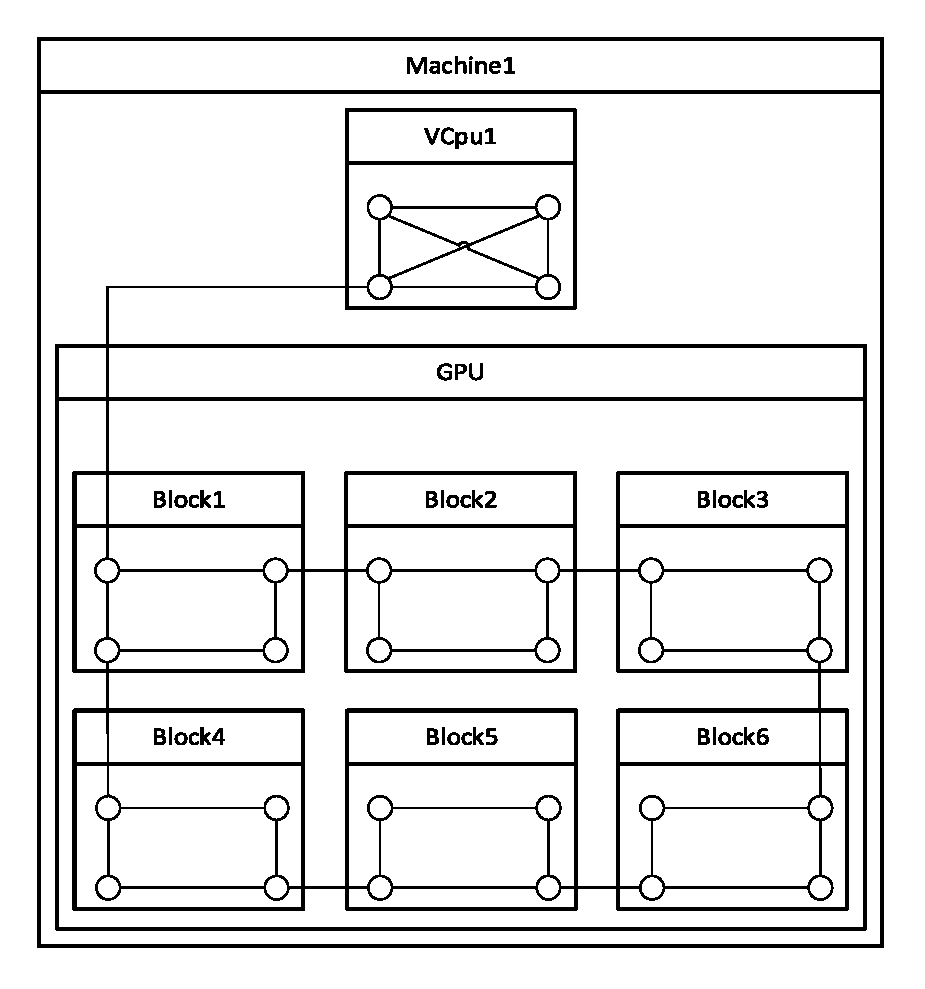
\includegraphics[scale=1]{klasterBbobWithGPU.pdf} 
 \caption{Struktura węzła obliczeniowego z rojem złożonym z 40 cząstek na CPU oraz 640 cząstek na GPU}
\end{figure}

\subsubsection{Klaster obliczeniowy}
W celu sprawdzenia zysku, jaki daje rozproszenie obliczeń na więcej węzłów obliczeniowych, zestawiliśmy do obliczeń dwa klastry - jeden złożony z 2 identycznych węzłów, drugi składający się z 4 identycznych węzłów. Na każdym węźle znajduje się rój złożony z 40 standardowych cząstek; żaden z węzłów nie korzysta z pomocy GPU.

\begin{figure}[H]
    \centering
    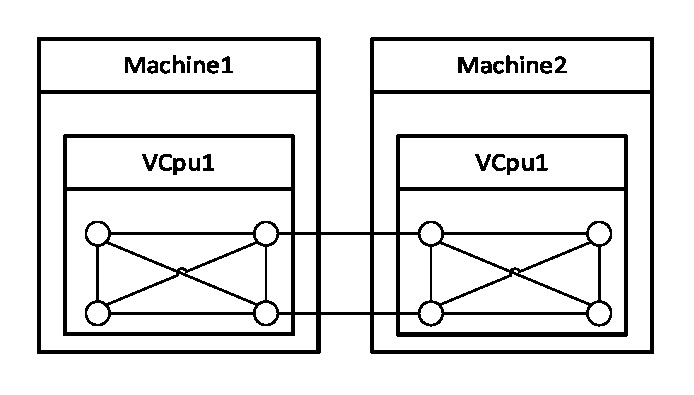
\includegraphics[scale=1]{klasterBbobNoGPU2Nodes.pdf} 
 \caption{Klaster obliczeniowy złożony z 2 węzłów}
\end{figure}

\begin{figure}[H]
    \centering
    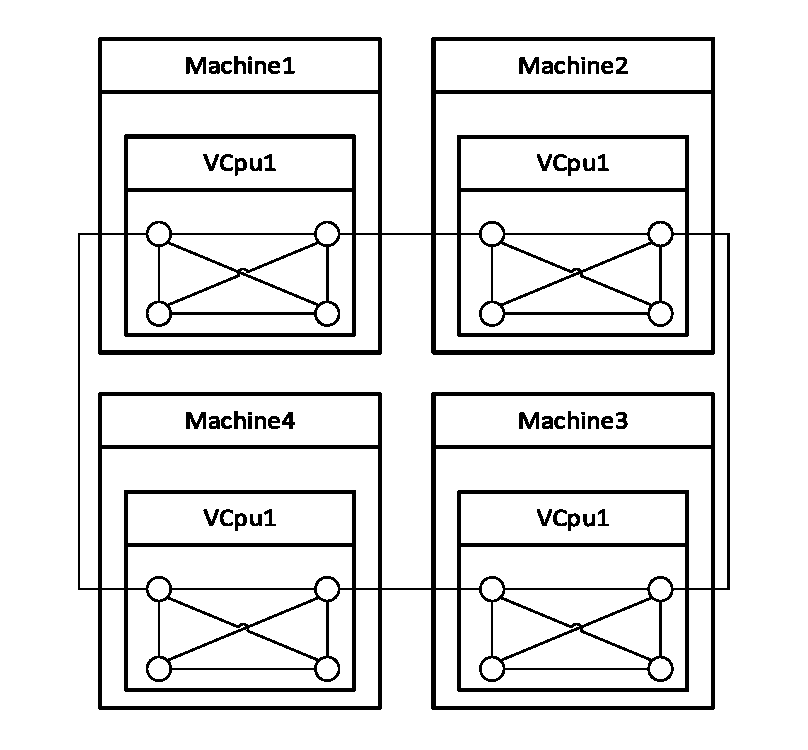
\includegraphics[scale=1]{klasterBbobNoGPU4Nodes.pdf} 
 \caption{Klaster obliczeniowy złożony z 4 węzłów}
\end{figure}

\section{Wyniki i ich interpretacja}

\subsection{Jak czytać}
Każdy z 24 typów funkcji celu posłużył do zbudowania 15 konkretnych instancji funkcji, różniących się przesunięciem względem początku układu współrzędnych, obrotem, rozciągnięciem lub inną prostą transformacją nie wpływającą na istotę problemu - wyniki dla tych instancji są następnie uśredniane i prezentowane jako wyniki dla danej funkcji celu. Dodatkowo dla każdej konkretnej instancji funkcji celu bierzemy pod uwagę różne progi odległości od optimum i prezentujemy liczbę funkcji, dla których choć w jednej instancji udało się osiągnąć odległość od optimum mniejszą niż $10^{1}$, $10^{-1}$, $10^{-4}$ oraz $10^{-8}$.

\subsection{Rezultaty}

\subsection{Standardowe PSO}
Otrzymane rezultaty standardowej wersji PSO na pojedynczym węźle obliczeniowym są zgodne z oczekiwaniami - algorytm radzi sobie dość dobrze z prostymi funkcjami przy niskiej liczbie wymiarów i szybko znajduje dal nich optimum z dużą dokładnością, jednakże dla funkcji trudnych, zwłaszcza w większym wymiarze, PSO osiąga bardzo niską skuteczność.

Przy interpretacji wyników najbardziej istotne dla nas było względne porównanie różnych konfiguracji, aby stwierdzić, czy przynoszą one zysk względem konfiguracji bazowej. Nie skupialiśmy się na bezwzględnych wynikach testów.

\begin{figure}[H]
    \centering
    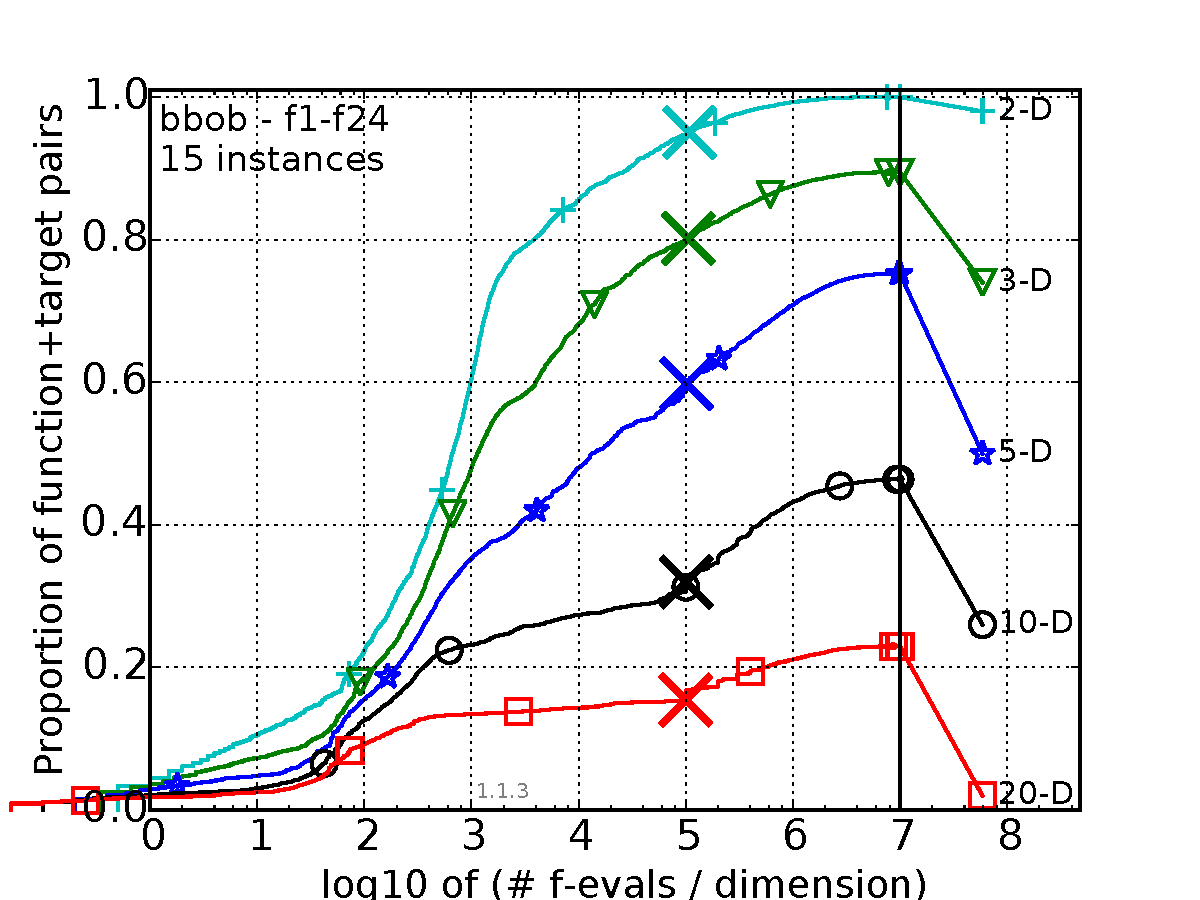
\includegraphics[scale=.75]{charts/1node40st.pdf} 
 \caption{Wyniki zbiorcze dla roju złożonego z 40 cząstek standardowych}
\end{figure}

\begin{figure}[H]
    \centering
    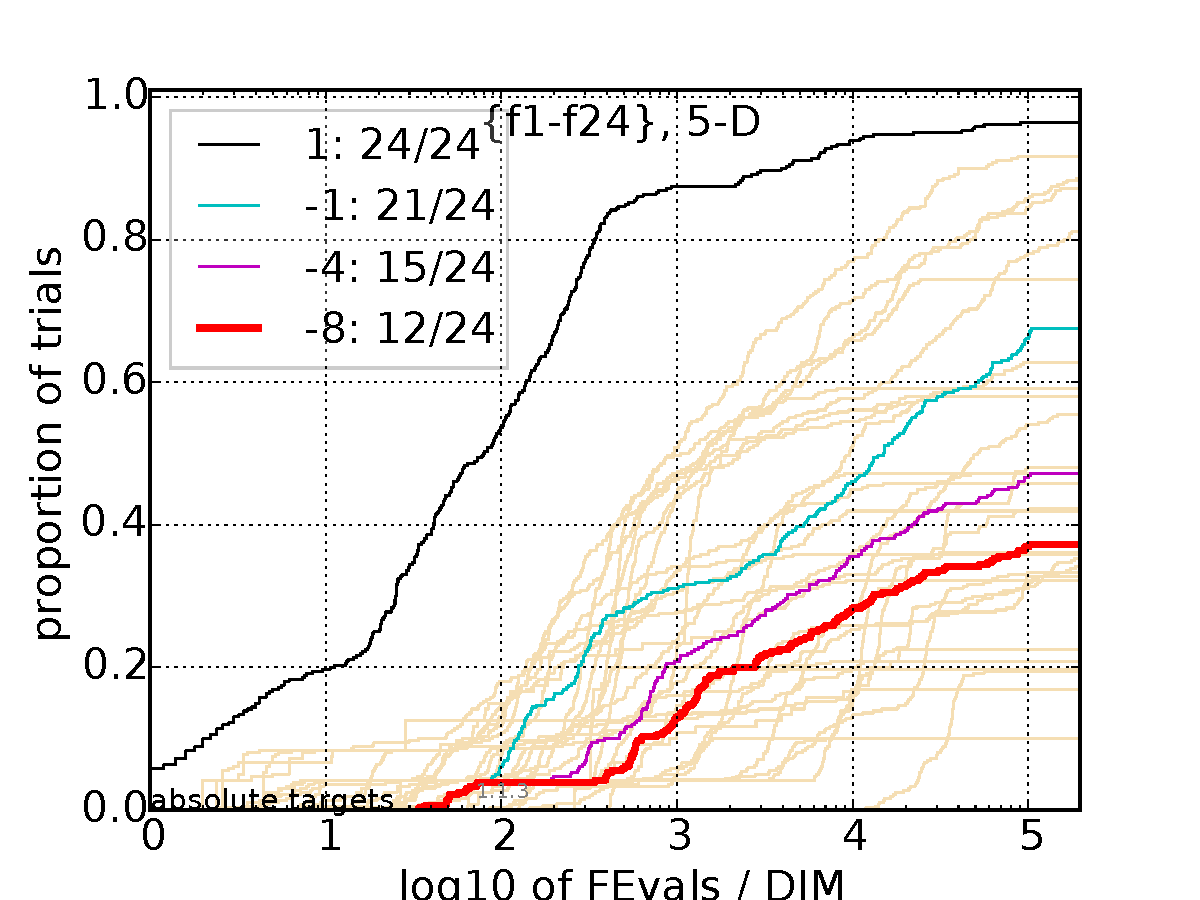
\includegraphics[scale=.75]{charts/1node40st_5D.pdf} 
 \caption{Wyniki dla roju złożonego z 40 cząstek standardowych dla funkcji pięciowymiarowych wraz z proporcją osiągniętych celów dla różnych progów dokładności}
\end{figure}

\subsection{Hybrydyzacja PSO}
Porównanie wyników standardowego PSO z wynikami uzyskanymi po zastąpieniu połowy cząstek roju cząstkami naładowanymi wskazuje niestety na jedynie niewielką poprawę działania, wyraźnie widoczną jedynie dla niektórych funkcji, takich jak funkcja sferyczna oraz funkcja Gallaghera oraz nieznaczne pogorszenie wyników w innych przypadkach. Charged PSO zostało pierwotnie stworzone z myślą o zastosowaniu w problemie optymalizacji dynamicznej, zaś w badanych przez nas scenariuszach sprawdza się bardzo podobnie do standardowego PSO.

\begin{figure}[H]
    \centering
    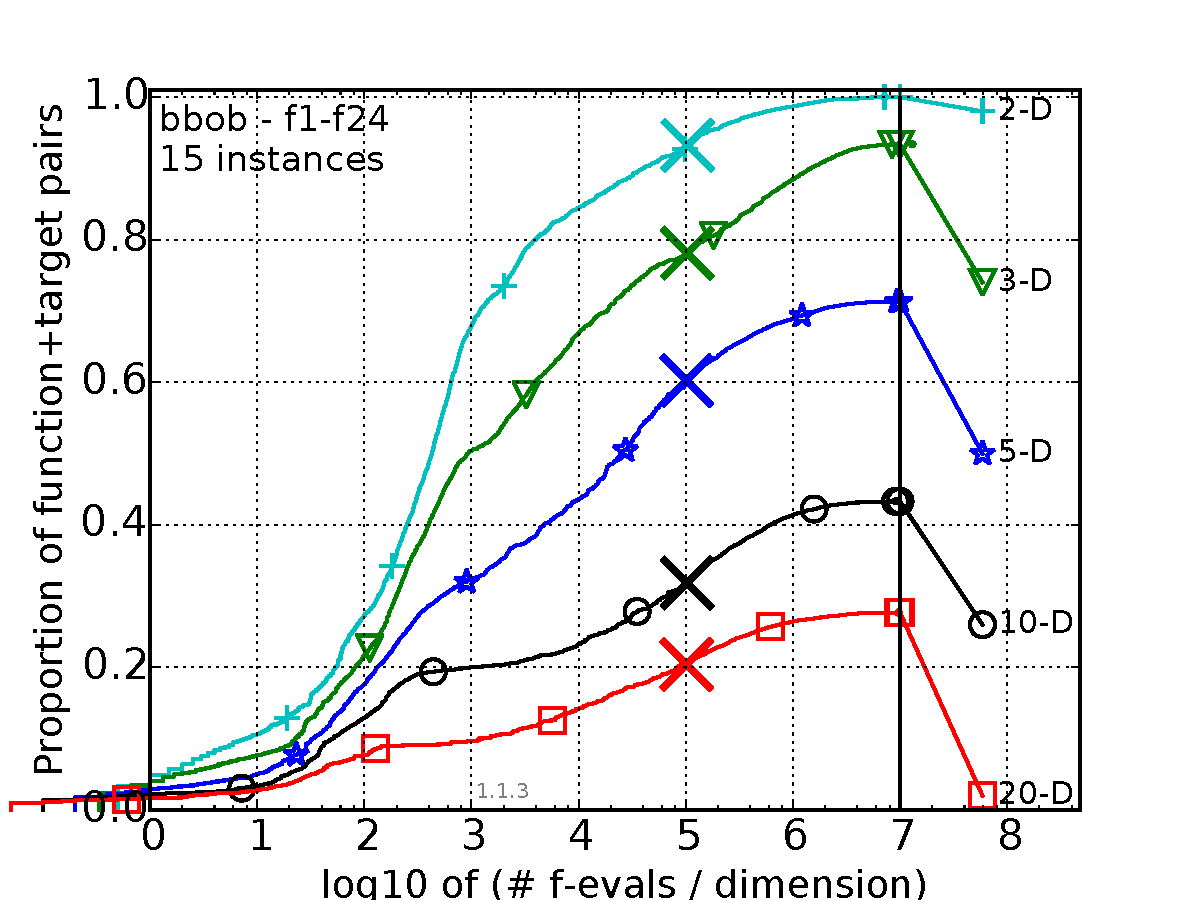
\includegraphics[scale=.75]{charts/1node20ch20st.pdf} 
 \caption{Wyniki zbiorcze dla roju złożonego z 20 cząstek standardowych i 20 cząstek naładowanych}
\end{figure}

\begin{figure}[H]
    \centering
    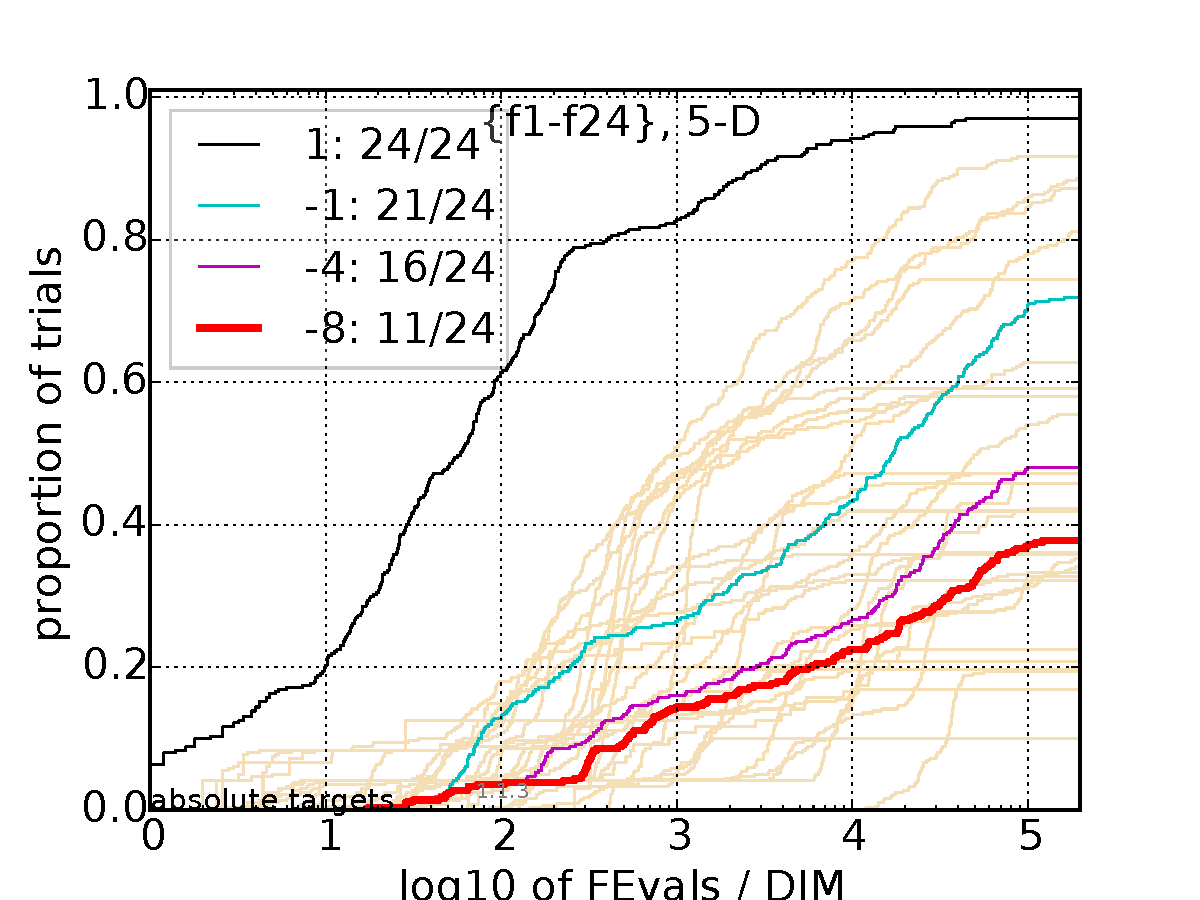
\includegraphics[scale=.75]{charts/1node20ch20st_5D.pdf} 
 \caption{Wyniki dla roju złożonego z 20 cząstek standardowych i 20 cząstek naładowanych dla funkcji pięciowymiarowych wraz z proporcją osiągniętych celów dla różnych progów dokładności}
\end{figure}

\subsection{Obliczenia na GPU}
Przy wykorzystaniu obliczeń na GPU zaobserwowaliśmy średnio jedynie nieznaczną poprawę jakości. Pomimo tego, że rój na karcie graficznej był 16-krotnie liczniejszy niż na CPU, fakt że implementował on najprostszą wersję PSO, nie wykorzystującą mechanizmu restartów cząstek, mógł odpowiadać za jego relatywnie niską skuteczność, pomimo, że wykonywał on między 2-, a 11-krotnie więcej ewaluacji dla każdej z funkcji testowych. Nieco bardziej zauważalna poprawa nastąpiła jedynie dla funkcji sferycznej oraz elipsoidalnej. 



\begin{figure}[H]
    \centering
    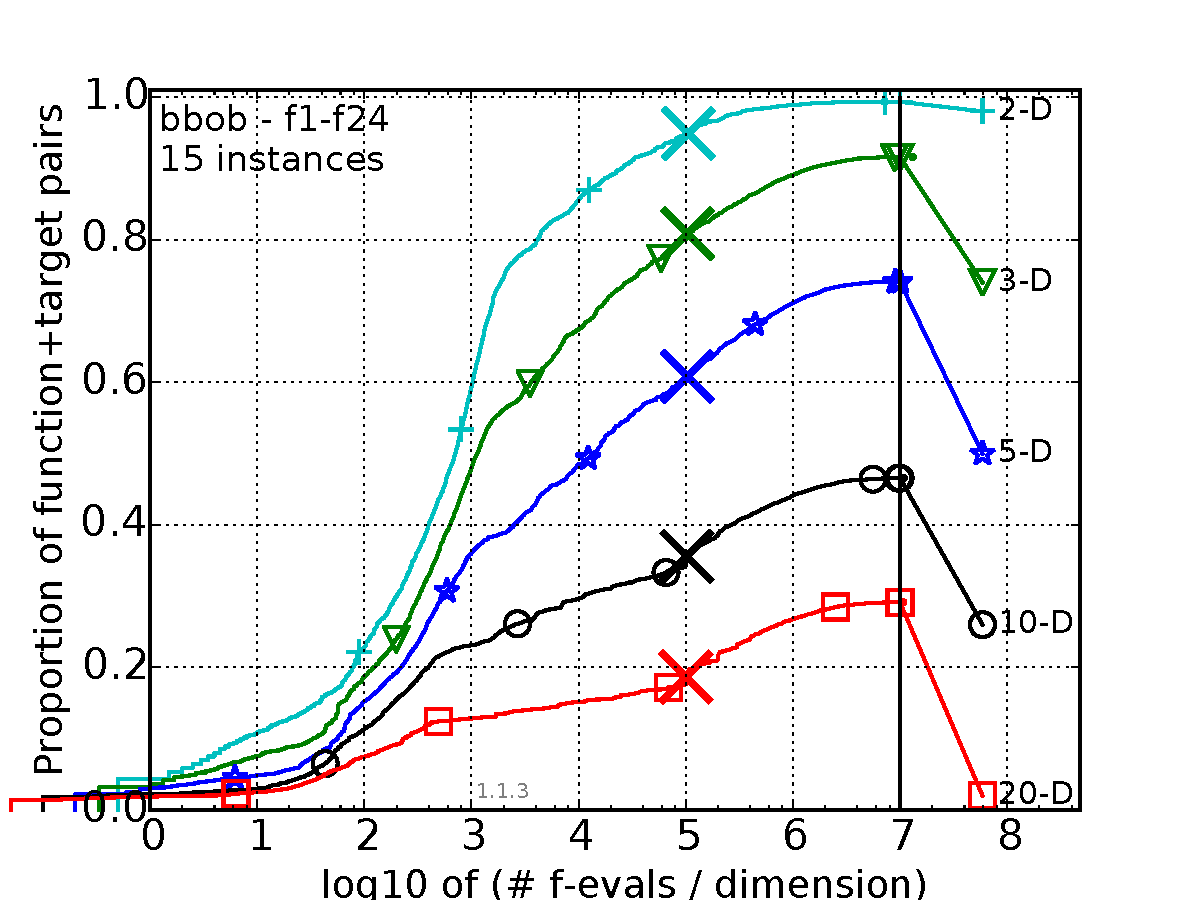
\includegraphics[scale=.75]{charts/1node40stGPU.pdf} 
 \caption{Wyniki zbiorcze dla roju złożonego z 40 cząstek standardowych i z uruchomioną jednostką GPU z 640 cząstkami}
\end{figure}

\begin{figure}[H]
    \centering
    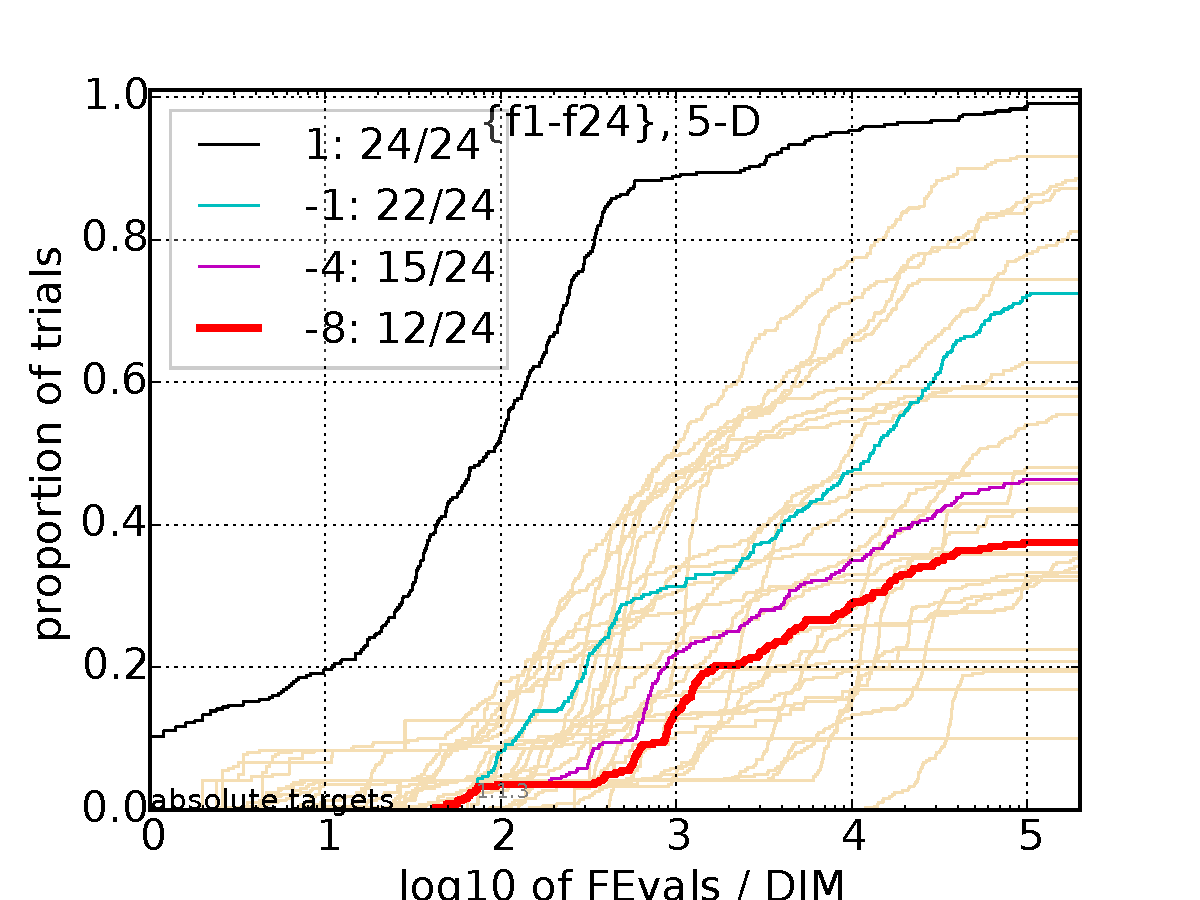
\includegraphics[scale=.75]{charts/1node40stGPU_5D.pdf} 
 \caption{Wyniki dla roju złożonego złożonego z 40 cząstek standardowych i z uruchomioną jednostką GPU z 640 cząstkami dla funkcji pięciowymiarowych wraz z proporcją osiągniętych celów dla różnych progów dokładności}
\end{figure}

% porównanie

\begin{figure}[H]
    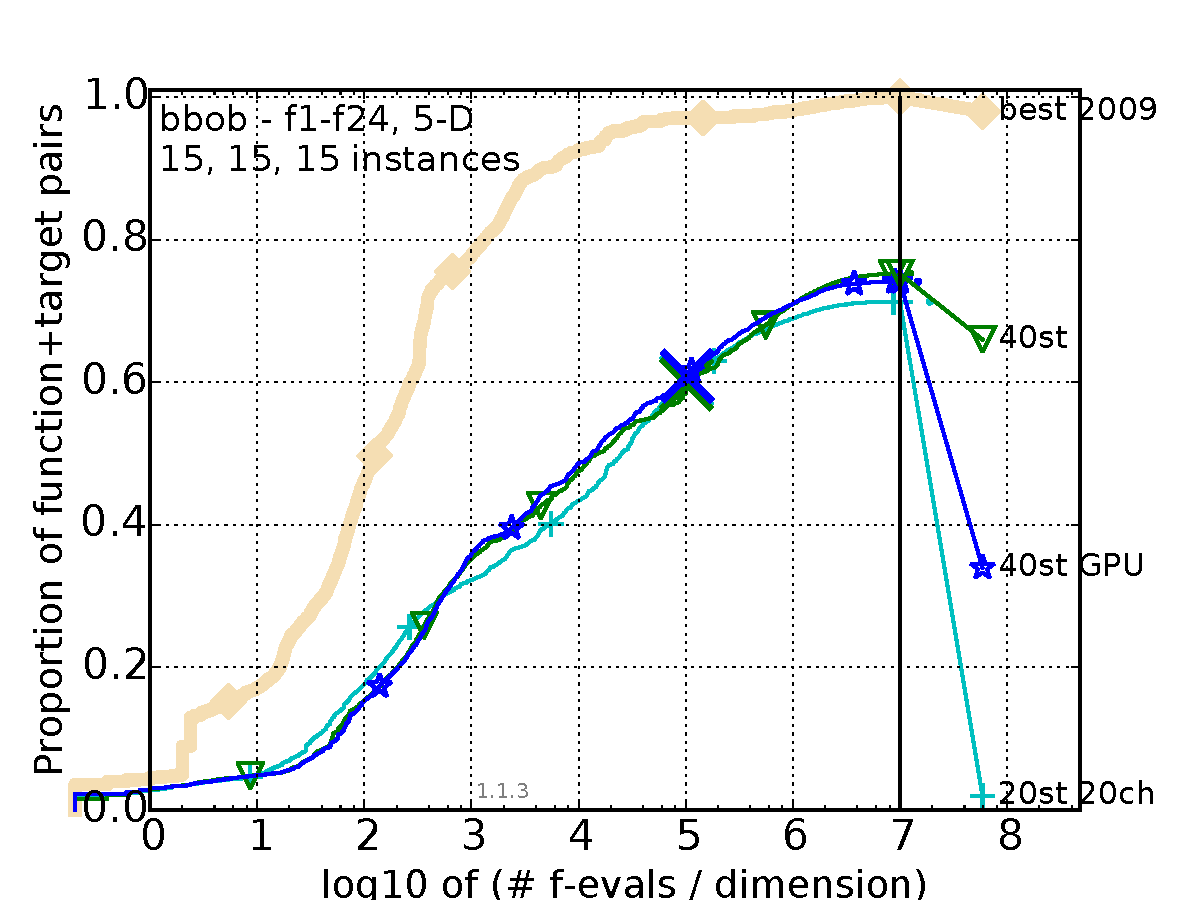
\includegraphics[scale=.75]{charts/1nodeCompare_5D.pdf} \par
 \caption{Wykres porównujący wyniki na pojedynczym węźle wersji standardowej z wersją z cząstkami naładowanymi oraz z wersją wykorzystującą GPU. Wskazuje na brak wyraźnych różnic pomiędzy różnymi wersjami algorytmu działającymi na jednym węźle.}
\end{figure}

\subsection{Obliczenia na klastrze}
Wykorzystanie obliczeń rozproszonych na klastrze obliczeniowym przyniosło widoczną poprawę wyników, tym większą, im więcej węzłów obliczeniowych zostało wykorzystanych do obliczeń. Poprawa widoczna jest dla każdego rodzaju funkcji.

\subsubsection{Klaster złożony z dwóch węzłów}

\begin{figure}[H]
    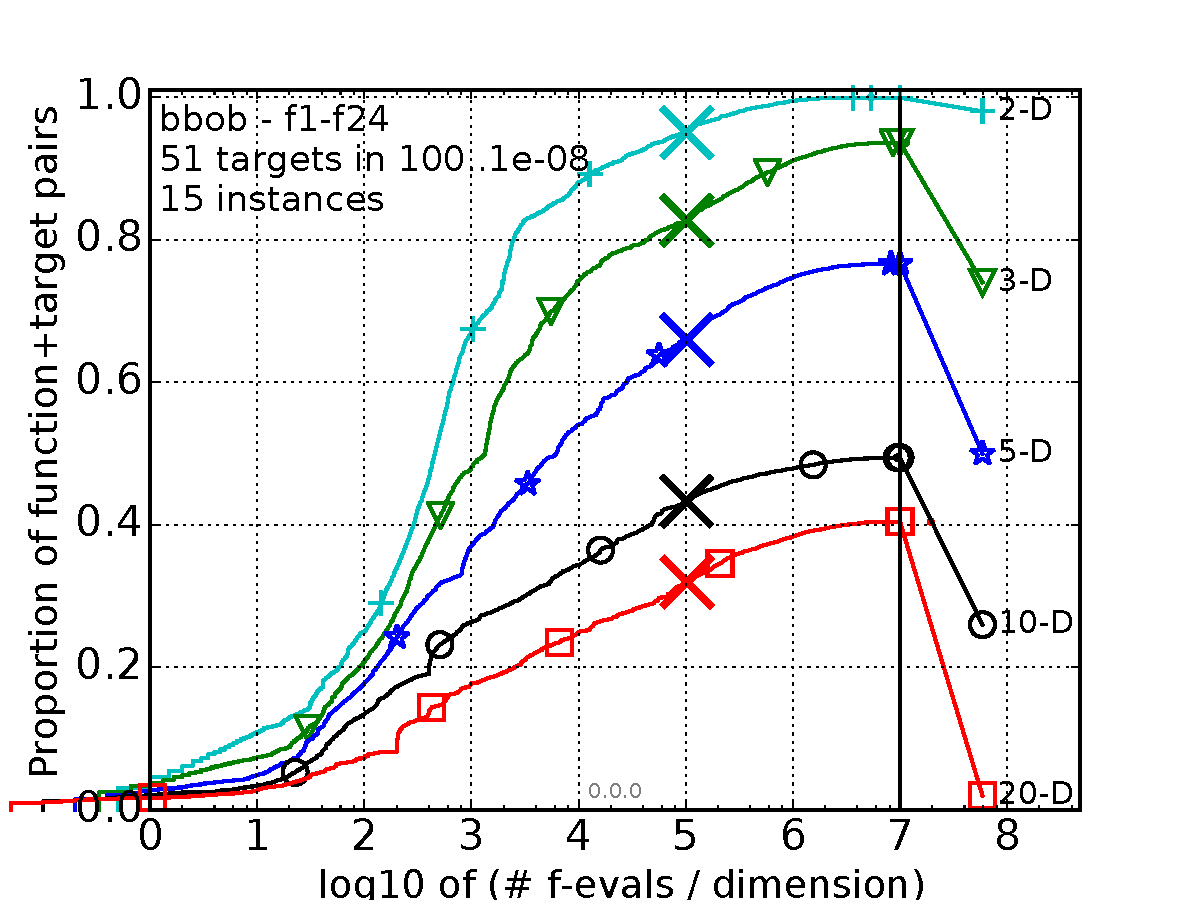
\includegraphics[scale=.75]{charts/2nodes.pdf} 
 \caption{Wyniki zbiorcze klastra zbudowanego z 2 węzłów}
\end{figure}

\begin{figure}[H]
    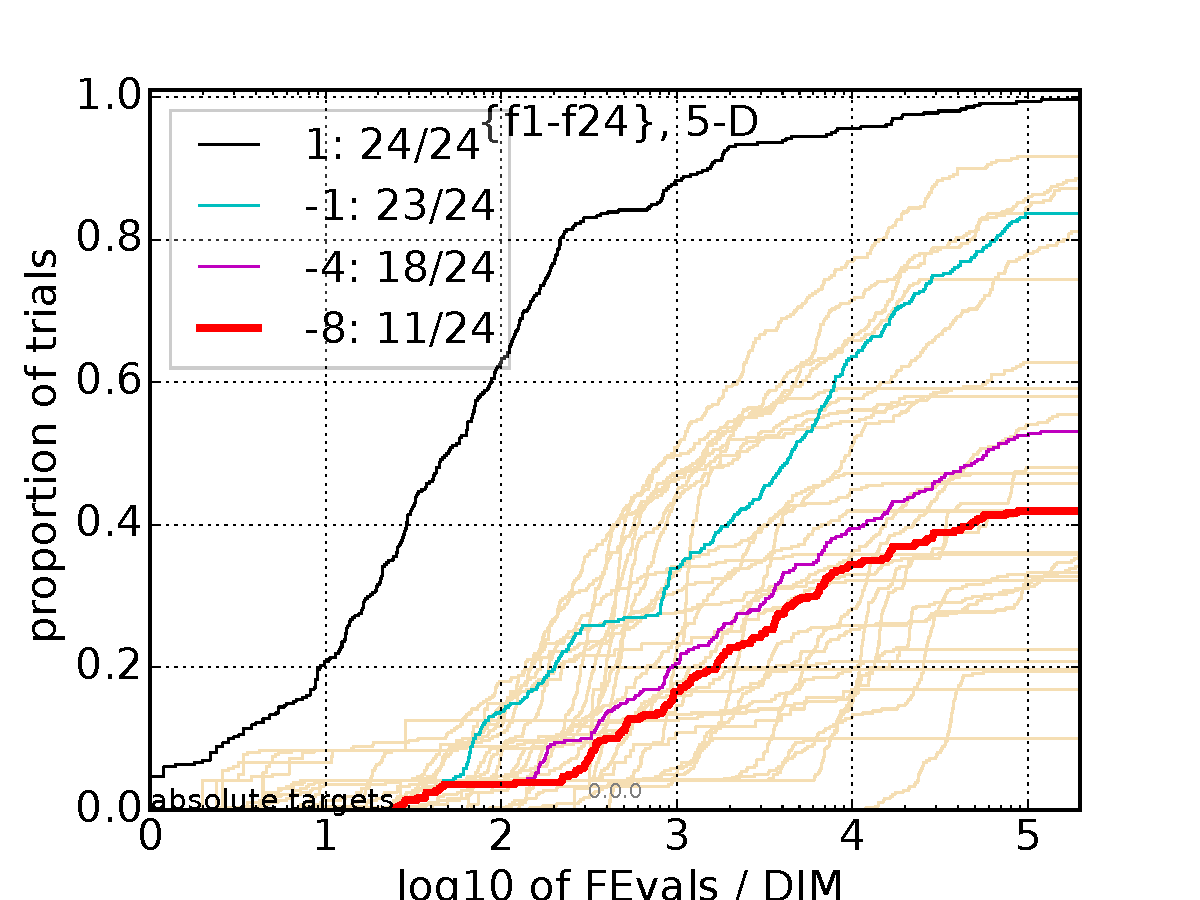
\includegraphics[scale=.75]{charts/2nodes_5D.pdf} 
 \caption{Wyniki klastra zbudowanego z 2 węzłów dla funkcji pięciowymiarowych wraz z proporcją osiągniętych celów dla różnych progów dokładności}
\end{figure}


\subsubsection{Klaster złożony z czterech węzłów}

\begin{figure}[H]
    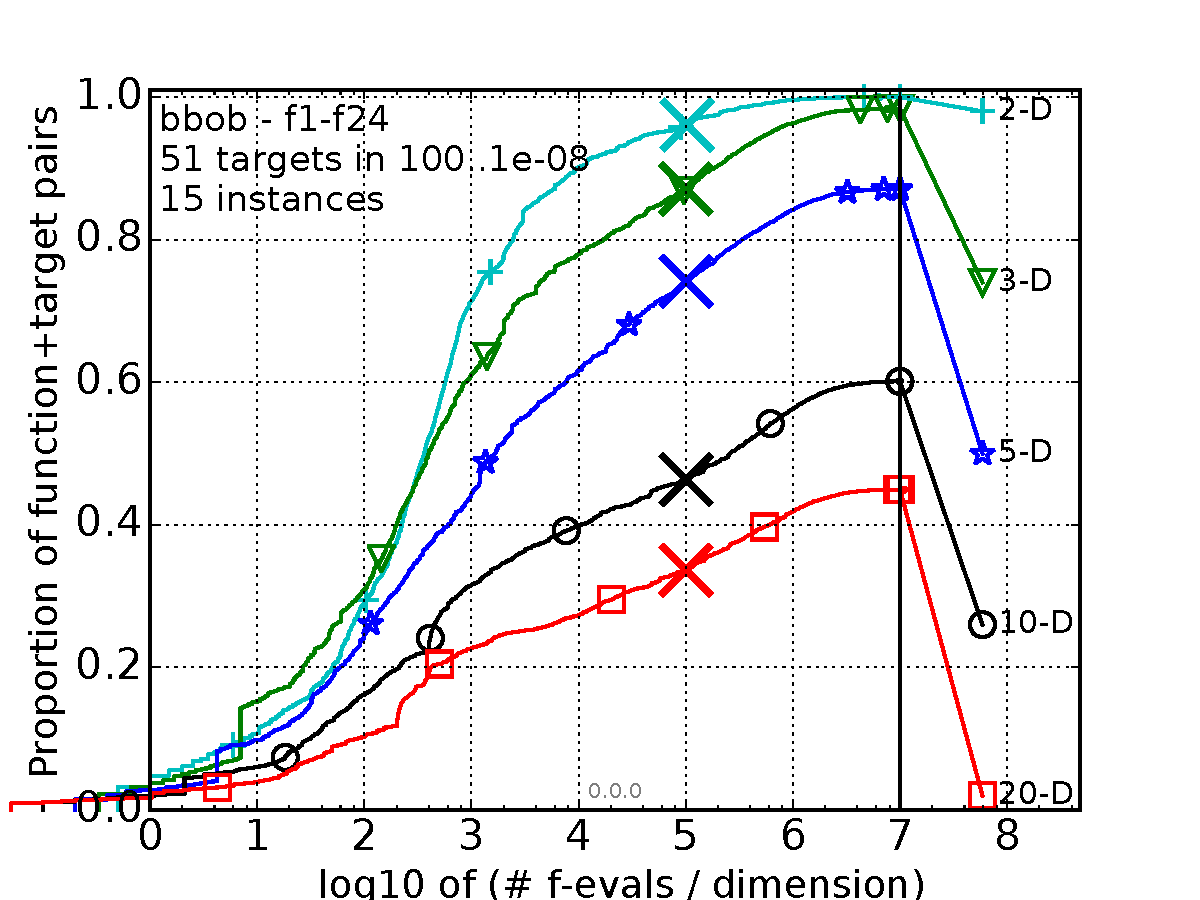
\includegraphics[scale=.75]{charts/4nodes.pdf} 
 \caption{Wyniki zbiorcze klastra zbudowanego z 4 węzłów}
\end{figure}

\begin{figure}[H]
    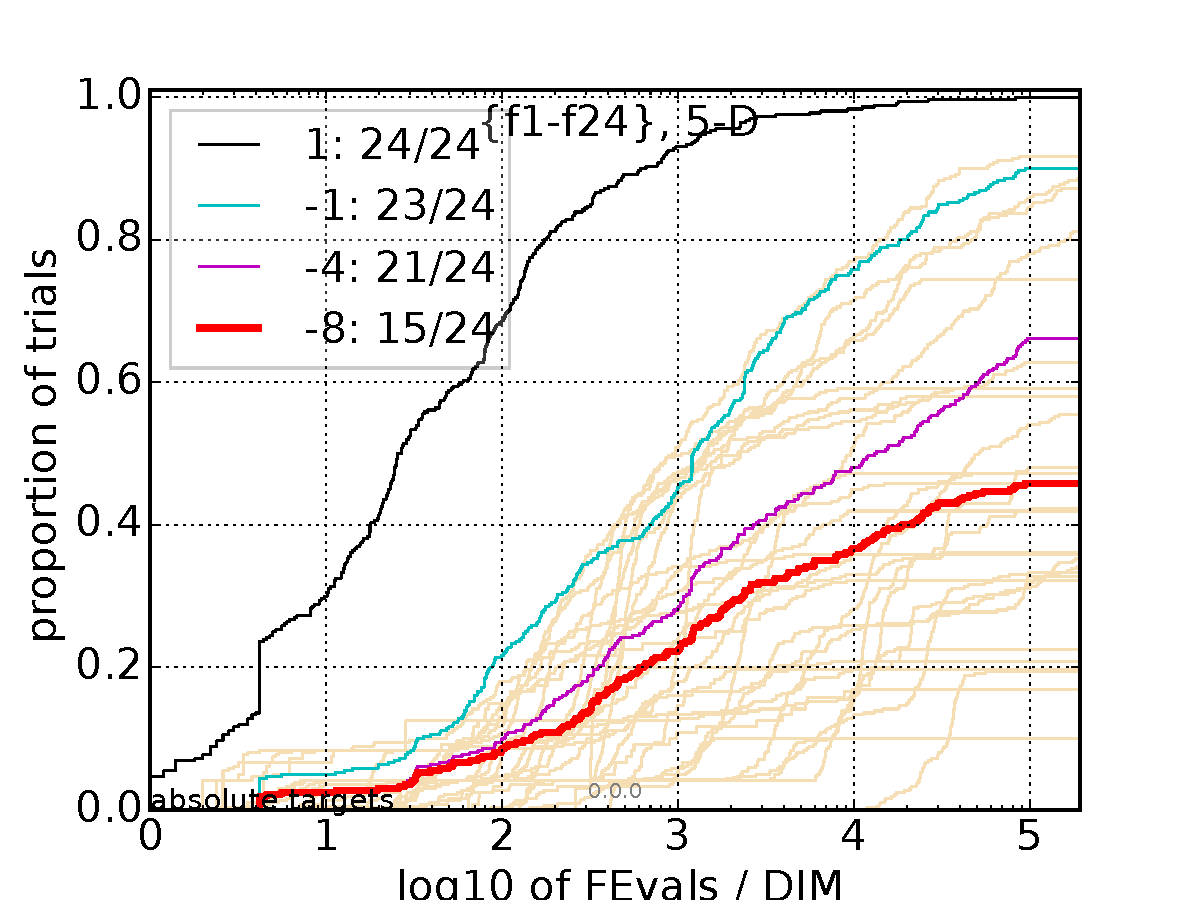
\includegraphics[scale=.75]{charts/4nodes_5D.pdf} \par
 \caption{Wyniki klastra zbudowanego z 4 węzłów dla funkcji pięciowymiarowych wraz z proporcją osiągniętych celów dla różnych progów dokładności}
\end{figure}

% porównanie

\begin{figure}[H]
    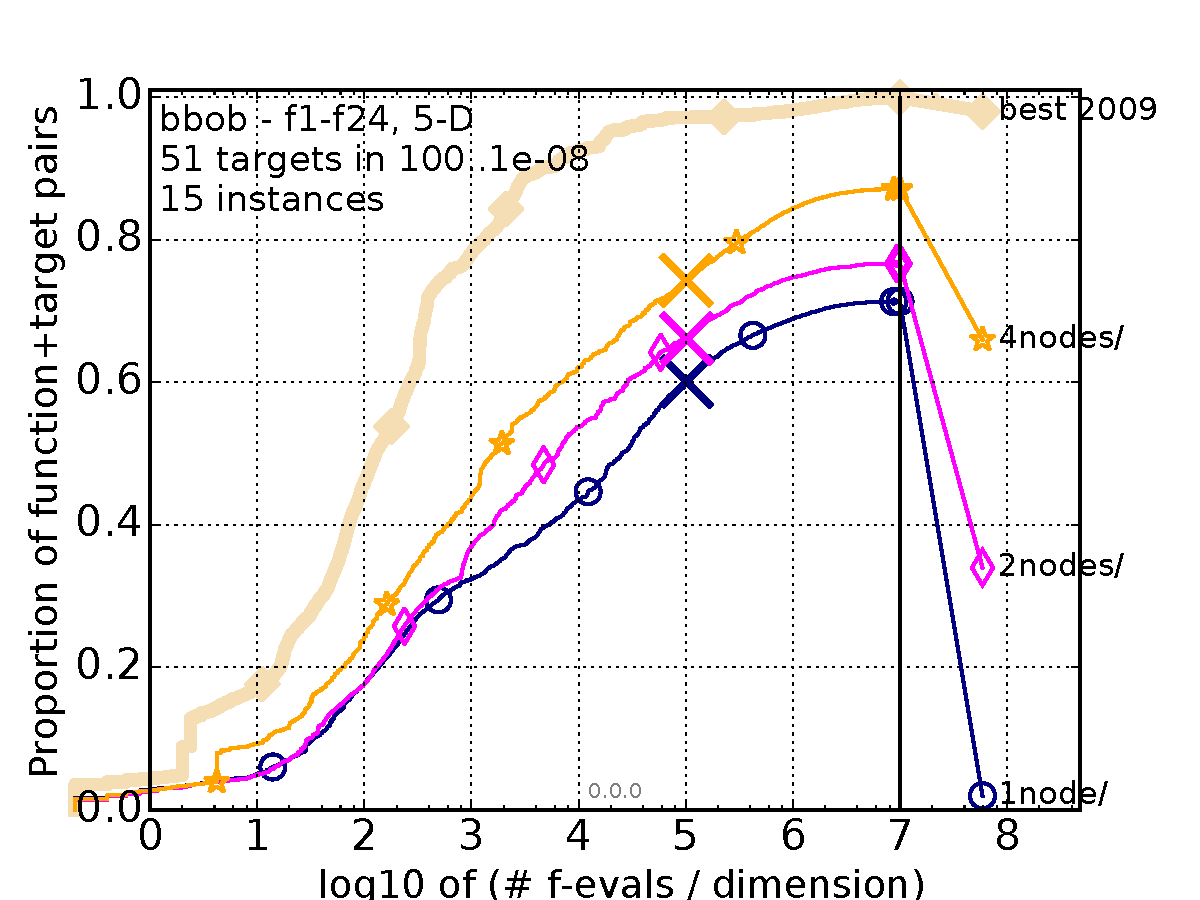
\includegraphics[scale=.75]{charts/124compare_5D.pdf} \par
 \caption{Wykres porównujący wyniki na pojedynczym węźle z wynikami klastra złożonego z 2 oraz z 4 węzłów. Można zauważyć poprawę wyników dla większej liczby węzłów obliczeniowych.}
\end{figure}


%%%%%%%%%%%%%%%%%%%%%%%%%%%%%%%%%%%%%%%%%%%%%%%%%%%%%%%%%%%%%%%%%%%%%

\chapter{Podział pracy}
Podział pracy prezentował się następująco:\\

\textbf{Paweł Kupidura} - Odpowiadał za implementację algorytmu w technologii CUDA oraz komunikację pomiędzy CPU a GPU. Dodatkowo stworzył pierwotną implementacją algorytmu PSO w C/C++.\\

\textbf{Hubert Rosiak} - Odpowiadał za stworzenie wrappera do platformy COCO. Brał udział w tworzeniu struktury węzła obliczeniowego.\\

\textbf{Kacper Trojanowski} - Brał udział w tworzeniu struktury klastra obliczeniowego i odpowiadał za zaprojektowanie komunikacji pomiędzy jego węzłami. Stworzył algorytm PSO w C\# umożliwiający jego łatwą modyfikację i hybrydyzację.

%%%%%%%%%%%%%%%%%%%%%%%%%%%%%%%%%%%%%%%%%%%%%%%%%%%%%%%%%%%%%%%%%%%%%

\chapter{Podsumowanie}

%1. o procesie produkcji
%	a. co było proste
%	b. co było trudne

%2. o produkcie końcowym
%	a. co się udało
%	b. co się nie udało

%3. o przyszłości
%	a. na jakim etapie projektu jesteśmy
%	b. co należałoby poprawić

Praca nad systemem do optymalizacji funkcji  okazała się być trudnym, ale pouczającym doświadczeniem. 

Implementacja algorytmu PSO na CPU, zarówno w wersji standardowej jak i zmodyfikowanej, nie stanowiła problemu - jedną z zalet algorytmu PSO jest jego prostota koncepcji i implementacji. Dzięki stworzeniu prostego interfejsu, mogliśmy w łatwy sposób wprowadzić do algorytmu modyfikacje, takie, jak np. hybrydyzacja z Charged PSO. Warto jednak wspomnieć, że zrezygnowaliśmy z początkowego pomysłu implementacji algorytmu w C/C++ na rzecz implementacji w języku C\#.

Trudniejszym zadaniem było napisanie algorytmu w technologii CUDA. Programowanie kart graficznych jest znacznie bardziej skomplikowane, toteż na GPU wyzwaniem okazało się już zaimplementowanie podstawowej wersji algorytmu i zapewnienie możliwości komunikacji roju cząstek na GPU z pozostałą częścią programu. Niemniej jednak, udało nam się zrealizować ten cel, wraz z pozostałymi założeniami początkowymi projektu, czyli, m.in. stworzeniem klastra obliczeniowego umożliwiającego jego uruchomienie w ramach obliczeń rozproszonych.

Klaster obliczeniowy spełnił swoje zadanie i w widoczny sposób poprawił wydajność naszego algorytmu optymalizacyjnego. Niestety implementacja PSO na karty graficzne, choć poprawna, nie przyniosła oczekiwanych rezultatów w postaci zysku czasowego, co prawdopodobnie wynika z zaimplementowania jedynie najprostszej wersji algorytmu oraz mało wydajnego procesu wymiany danych pomiędzy CPU a GPU. 

Zaadresowanie tych problemów powinno być kolejnym krokiem w procesie udoskonalania systemu. 

Wyzywaniem samym w sobie okazało się również przetestowanie naszego systemu optymalizacyjnego na zestawie benchmarków BBOB. Platforma testująca COCO, której w tym celu użyliśmy, napisana została w języku C, toteż wymagała stworzenie odpowiedniego wrappera umożliwiającego dostęp do niej z poziomu języka C\#.

%%%%%%%%%%%%%%%%%%%%%%%%%%%%%%%%%%%%%%%%%%%%%%%%%%%%%%%%%%%%%%%%%%%%%

\chapter{Słownik}

\textbf{Algorytm optymalizacyjny} - Algorytm rozwiązujący problem optymalizacji.\\
\textbf{Benchmark} - Sposób oceny jakości sprzętu lub programu komputerowego polegający na uruchomieniu zestawu testów i porównaniu ich ze znanymi standardami.\\
\textbf{BBOB} - Black-Box Optimization Benchmarking. Warsztaty na temat optymalizacji odbywające się podczas konferencji Genetic and Evolutionary Computation Conference (GECCO).\\
\textbf{Black-box optimization} - Rodzaj zadania optymalizacyjnego, w którym algorytm optymalizacyjny nie zna postaci funkcji celu, a może jedynie zapytać się o jej wartość w danym punkcie.\\
\textbf{COCO} - COmparing Continuous Optimisers. Platforma do porównywania algorytmów optymalizacyjnych.\\
\textbf{CUDA} - Platforma programistyczna firmy NVIDIA umożliwiająca wykorzystywanie procesorów graficznych w obliczeniach\\
\textbf{Framework} - Platforma programistyczna. Szkielet aplikacji definiujący jej ogólną strukturę i mechanizm działania lub dostarczający komponenty wykonujące określone zadania.\\
\textbf{Funkcja celu} - Funkcja, której ekstremum jest poszukiwane w zagadnieniu optymalizacji.\\
\textbf{GPU} - Graphics Processing Unit. Wyspecjalizowana jednostka obliczeniowa typu SIMD przystosowana do efektywnego przetwarzania grafiki komputerowej. Może być również wykorzystywana do obliczeń równoległych na dużych zbiorach danych.\\
\textbf{Klaster obliczeniowy} - Zespół węzłów obliczeniowych połączonych ze sobą siecią, umożliwiający prowadzenie wspólnych obliczeń.\\
\textbf{Obliczenia rozproszone} - Obliczenia prowadzone jednocześnie na wielu jednostkach obliczeniowych, mogących różnić się między sobą architekturą i położeniem geograficznym, ale komunikujących się ze sobą i mogących korzystać ze wspólnych zasobów. Synchronizacja między jednostkami zachodzi w szerszej skali niż w przypadku obliczeń równoległych.\\
\textbf{Obliczenia równoległe} - Zsynchronizowane obliczenia prowadzone jednocześnie na kilku jednostkach obliczeniowych, zazwyczaj procesorach na jednej maszynie.\\
\textbf{Optymalizacja} - Zagadnienie znajdowania wartości ekstremalnej (najczęściej minimalnej lub maksymalnej) zadanej funkcji celu.\\
\textbf{PSO} - Particle Swarm Optimization. Populacyjny algorytm optymalizacyjny, wykorzystujący populację cząstek poruszających się w przestrzeni możliwych rozwiązań.\\
\textbf{WCF} - Windows Communication Foundation. Platforma programistyczna wykorzystywana przy budowie aplikacji korzystających z komunikacji sieciowej.\\
\textbf{Wrapper} - Zestaw funkcji i klas mających za zadanie pośredniczenie między dwiema różnymi warstwami aplikacji.\\


%-----------Koniec części zasadniczej-----------

\begin{thebibliography}{11}

%Evolving Objects

\bibitem{EObjGeneral} M. Keijzer, J. J. Merelo, G. Romero, M. Schoenauer, \emph{Evolving Objects: a general purpose evolutionary computation library}, http://geneura.ugr.es/~jmerelo/habilitacion2005/papers/53.pdf

\bibitem{EOlib} \emph{Evolving Objects homepage}, http://eodev.sourceforge.net/

%COCO

\bibitem{Coco} \emph{COCO homepage}, http://coco.gforge.inria.fr

\bibitem{CocoPlatform} N. Hansen, A. Auger, O. Mersmann, T. Tusar, D. Brockhoff, \emph{COCO: a platform for comparing continuous optimizers in a black-box setting}, https://arxiv.org/pdf/1603.08785.pdf

%%

\bibitem{NewPso} R. C. Eberhart, J. Kennedy, \emph{A new optimizer using particle swarm theory}, Proc. 6th Int. Symp. Micromachine Human Sci., Nagoya, Japan, 1995, pp. 39-43

\bibitem{Pso} J. Kennedy, R. C. Eberhart, \emph{Particle swarm Optimization}, Proc. IEEE Int. Conf. Neural Networks, 1995, pp. 1942-1948

\bibitem{SPso} Maurice Clerc, \emph{Standard particle swarm optimisation. From 2006 to 2011}, http://clerc.maurice.free.fr/pso/SPSO\_descriptions.pdf

\bibitem{PSO_2D_img} Randy Olson, \emph{Visualization of two dimensions of a NK fitness landscape}, 2013, URL https://commons.wikimedia.org/wiki/ \\ File:Visualization\_of\_two\_dimensions\_of\_a\_NK\_fitness\_landscape.png., [Online; dostęp grudzień 2016]

%z Comprehensive Learning PSO...

\bibitem{ComprLearnPso} J. J. Liang, A. K. Qin, P. N. Suganthan, S. Baskar, \emph{Comprehensive learning particle swarm optimizer for global optimization of multimodal functions}, IEEE Transactions on Evolutionary Computation, Vol. 10, No. 3, June 2006

\bibitem{ModPsoInertia} Y. Shi, R. C. Eberhart, \emph{A modified particle swarm optimizer}, Proc. IEEE Congr. Evol. Comput., 1998, pp. 69-73

\bibitem{ParamSelPso} Y. Shi, R. C. Eberhart, \emph{Parameter selection in particle swarm optimization}, Proc. 7th Conf. Evol. Programming, New York, 1998, pp. 591-600

\bibitem{PsoFuzzyInertia} Y. Shi, R. C. Eberhart, \emph{Particle swarm optimization with fuzzy adaptive inertia weight}, Proc. Workshop Particle Swarm Optimization, Indianapolis, IN, 2001, pp. 101-106

\bibitem{SelfOrgHPso} A. Ratnaweera, S. Halgamuge, H. Watson, \emph{Self-organizing hierarchical particle swarm optimizer with time varying accelerating coefficients}, IEEE Trans. Evol. Comput., vol. 8, pp. 240-255, Jun. 2004

\bibitem{VmaxPso} H. Y. Fan, Y. Shi, \emph{Study on Vmax of particle swarm optimization}, Proc. Workshop Particle Swarm Optimization, Indianapolis, IN, 2001

\bibitem{TopologyPso} J. Kennedy, \emph{Small worlds and mega-minds: Effects of neighborhood topology on particle swarm performance}, Proc. Congr. Evol. Comput., 1999, pp. 1931-1938

\bibitem{PopStructPso} J. Kennedy, R. Mendes, \emph{Population structure and particle swarm performance}, Proc. IEEE Congr. Evol. Comput., Honolulu, HI, 2002, pp. 1671-1676

\bibitem{PsoNeighOp} P. N. Suganthan, \emph{Particle swarm optimizer with neighborhood operator}, Proc. Congr. Evol. Comput., Washington, DC, 1999, pp. 1958-1962

\bibitem{MultiobjDynNeighPso} X. Hu, R. C. Eberhart, \emph{Multiobjective optimization using dynamic neighborhood particle swarm optimization}, Proc. Congr. Evol. Comput., Honolulu, HI, 2002, pp. 1677-1681

\bibitem{UPso} K. E. parsopoulos, M. N. Vrahatis, \emph{UPSO-A unified particle swarm optimization scheme}, Lecture Series on Computational Sciences, 2004, pp. 868-873

\bibitem{FullyInformedPso} R. Mendes, J. Kennedy, J. Neves, \emph{The fully informed particle swarm: Simpler, maybe better}, IEEE Trans. Evol. Comput., vol. 8, pp. 204-210, Jun. 2004

\bibitem{FitnessDistRatio} T. Peran, K. Veeramachaneni, C. K. Mohan, \emph{Fitness-distance-ratio based particle swarm optimization}, Proc. Swarm Intelligence Symp., 2003, pp. 174-181

\bibitem{SelectionPso} P. J. Angeline, \emph{Using selection to improve particle swarm optimization}, Proc. IEEE Congr. Evol. Comput., Anchorage, AK, 1998, pp. 84-89

\bibitem{HybridPsoBreedingSubpop} M. Lovbjerg, T. K. Rasmussen, T. Krink, \emph{Hybrid particle swarm optimizer with breeding and subpopulations}, Proc. Genetic Evol. Comput. Conf., 2001, pp. 469-476

\bibitem{EPso} V. Miranda, N. Fonseca, \emph{New evolutionary particle swarm algorithm (EPSO) applied to voltage/VAR control}, Proc. 14th Power Syst. Comput. Conf., Seville, Spain, 2002. [Online]. Available: http://www.pscc02.org/papers/s21pos.pdf

\bibitem{PsoCriticality} M. Lovbjerg, T. Krink, \emph{Extending particle swarm optimizers with self-organized criticality}, Proc. Congr. Evol. Comput., Honolulu, HI, 2002, pp. 1588-1593

\bibitem{CollisionAvoiding} T. M. Blackwell, P. J. Bentley, \emph{Don't push me! Collision-avoiding swarms}, Proc. IEEE Congr. Evol. Comput., Honolulu, HI, 2002, pp. 1691-1696

\bibitem{DissipativePso} X. Xie, W. Zhang, Z. Yang, \emph{A dissipative particle swarm optimization}, Proc. Congr. Evol. Comput., Honolulu, HI, 2002, pp. 1456-1461

\bibitem{ComputGlobOptPso} K. E. Parsopoulos, M. N. Vrahatis, \emph{On the computation of all global minimizers through particle swarm optimization}, IEEE Trans. Evol. Comput., vol. 8, pp. 211-224, Jun. 2004

%z Comparison of parallel PSO...

\bibitem{ComparisonParallelGpuPso} V. Roberge, M. Tarbouchi, \emph{Comparison of parallel particle swarm optimizers for graphical processing units and multicore processors}, International Journal of Computational Intelligence and Applications, Vol. 12 No. 1 (2013)

\bibitem{ComparGpuPso} G. A. Laguna-Sanchez, M. Olguin-Carbajal, N. Cruz-Cortes, R. Barron-Fernandez, J. Alvarez-Cedillo, \emph{Comparative study of parallel variants for a particle swarm optimization algorithm implemented on a multithreading GPU}, J. Appl. Res. Technol. 7(3) (2010) 292-309

\bibitem{BlockOccupancyGpu} M. Cardenas-Montes, M. Vega-Rodriguez, J. Rodriguez-Vazquez, A. Gomez-Iglesias, \emph{Effect of the block occupancy in GPGPU over the performance of particle swarm algorithm}, Proc. 10th Int. Conf. Adaptive and Natural Computing Algorithms, Vol. 1 (Springer Berlin, Heidelberg, 2011), pp. 310-319

%Accelerating parallel..

\bibitem{AccelParallelPso} Y. Hung, W. Wang, \emph{Accelerating parallel particle swarm optimization via GPU}, 2012, Optimization Methods and Software, 27:1, 33-51, http://dx.doi.org/10.1080/10556788.2010.509435

\bibitem{Pso8} M. Clerc, \emph{Particle swarm optimization}, ISTE Publishing Company, Newport Beach, CA, 2006

\bibitem{PsoCuda} L. Mussi, S. Cagnoni, \emph{Particle swarm optimization within the CUDA architecture}, 2009, Availabe: http://www.gpgpgpu.com/gecco2009/1.pdf.

\bibitem{CudaProgGuide} NVIDIA Corporation, \emph{NVIDIA CUDA Programming Guide}, Version 2.3.1, 2009

\bibitem{GpuBasedPso} Y. Zhou, Y. Tan, \emph{GPU-based parallel particle swarm optimization}, IEEE Congress on Evolutionary Computation, 2009, pp. 1493-1500

\bibitem{PsoGraphHardLocPat} W. Zhu, J. Curry, \emph{Particle swarm with graphics hardware acceleration and local pattern search on bound constrained problems}, IEEE Swarm Intelligence Symposium (SIS '09), 2009, pp. 1-8

\end{thebibliography}
%\tableofcontents
\clearpage
\pagestyle{empty}
\noindent Warszawa, dnia ...............
\vspace{5cm}
\begin{center}
\LARGE{Oświadczenie}
\end{center}
Oświadczamy, że moją część pracy inżynierskiej pod tytułem: ,,Efektywna implementacja wybranego algorytmu optymalizacji globalnej'', której promotorem jest mgr inż. Michał Okulewicz, wykonałem samodzielnie, co poświadczam własnoręcznym podpisem.
\vspace{2cm}
\begin{flushright}
...........................................
\end{flushright}
\end{document}